\chapter{Metadata Visualization}
\label{chapter:metadata-visualization}
\graphicspath{{figs/03-visualization/}}

Among the presented tools in chapter \ref{chapter:background}, MONTRA was our go-to mainly because of its data source-centric approach.
Also, no real data is shown here, only metadata is handled within the platform.
Yet, it still allows imposing access permissions at several levels.

This chapter will detail the crucial concepts of the MONTRA framework and its internal data model, followed by the description of the refactoring process that was done to the platform, with improvements and its flaws fixed.

\section{MONTRA}
% O que é o montra e o seu estado atual
% explicar de maneira mais aprefundada a paltaforma, realçando partes que devem ser alteradas ou que não estão corretas

Originally, the MONTRA framework was developed by the Bioinformatics team of the Institute of Electronics and Informatics Engineering of Aveiro associated with the \gls{emif} project with the goal to develop a common patient health information framework with emphasis on the research topics of Obesity and its metabolic complications and Markers for the development of Alzheimer's disease and other dementias.
The code is publicly available on github\footnote{https://github.com/bioinformatics-ua/montra}, whereby Django 1.4, a high-level Python Web framework\cite{django}, was used as a framework to develop the entire system.
This framework allows to develop complete web applications, in a faster and easier way.
It contains a model layer that allows specifying database tables through python classes called models, following a \gls{orm} approach, allowing to perform database queries through python code instead of \gls{sql} queries.
Django can then check if there are new models or if existing ones have changed. Such changes are expressed through database migration files which will apply them to the database tables.
Next, the developer can set custom URL patterns so specific requests are handled by a specific function of the view layer, where the business logic will be implemented.
Finally, Django contains a template layer that allows building dynamic \gls{html} pages without requiring to have a separate javascript framework to do such.
The developer builds the main static structure of the page and then uses a special syntax that describes how Django should display the data received from the view layer.
Django also has an important form feature that allows to easily create a set of pages that allow performing the usual \gls{crud} operation over the database model.

MONTRA's development started at the beginning of 2013 and ended in the middle of 2018.
After this, at the end of 2018, the framework was adopted by the \gls{ehden} project, to develop a portal to allow discovery and analysis of health data on their network of data sources.
Currently, the project is being developed in a private repository but intends to make it public after the code base is more robust and well documented.

\subsection{Communities}

In the first versions of the framework, MONTRA allowed only one level of organization related to data sources, in which they could only be separated according to their skeleton that describe their original data, which will be more detailed in the next subsection.
Newer versions created the concept of a Community.
This allows having multiple networks of data sources on the same portal, where originally the only option was to have different installations of the framework.

These communities can be created in several ways:

\begin{enumerate}
    \item the admin can create it through Django's admin console;
    \item a user can request a community to be created through a form and then the admin will receive an admin with such request;
    \item the MONTRA installation can be deployed in a single community mode where only one community exists, which is created on the first setup, giving the idea that there is no community concept on the platform.
\end{enumerate}

They also can have different access levels:

\begin{itemize}
    \item Open: Does not require membership. Any user can access the data sources of this community;
    \item Public: Does not require a membership however, the user needs to accept a set of terms and conditions before being able to access the data sources;
    \item Moderated: A user has to request the community managers for approval;
    \item Invitation: Users can only access and see the community by invite and subsequent approval.
\end{itemize}

\subsection*{Plugins}
The concept of Community also allows customization at that level, affecting only sections within that given community.
One example of such customization is plugins, a way to extend the functionalities of the framework without having to deal with the base code.
These plugins can either be full web applications, with different functionalities, that are linked to MONTRA through the community navigation menu or extensions that provide extra data services such as a dashboard about the data of a data source.

\subsection{Questionnaires}
% questions
% tipo de questoes

As the data from different data sources is highly heterogeneous, MONTRA ensures that the data inserted within a given community follow a common structure.
This structure is called a skeleton, which is represented in a form of a questionnaire with a set of questions, which can then be grouped in sections called Question Sets.
It represents a set of metadata that better describes the original data of data sources that need to remain private.
The skeleton schema can easily be defined through a spreadsheet, which will be more detailed on subsection \ref{subsection:excel}.

Next is presented the available question types which can be used to build a questionnaire for a community

\begin{longtable}[c]{|c|c|}
\hline
\textbf{Type}                     & \textbf{Description}                                        \\ \hline
\endhead
choice                            & Single choice (radio box)                                   \\ \hline
choice-freeform                   & Single choice with an open text fields                      \\ \hline
choice-multiple                   & Multiple choice (checkbox)                                  \\ \hline
choice-multiple-freeform          & Multiple choice with and open text fields                   \\ \hline
choice-multiple-freeform-options  & Multiple choice with and open text fields                   \\ \hline
choice-tabular                    & Creates a table with single, multiple choices or text by row      \\ \hline
choice-yesno                      & Single choice with yea and no choices                       \\ \hline
choice-yesnodontknow              & Single choice with yes, no and do not know choices          \\ \hline
comment                           & Used to separate groups of questions                        \\ \hline
custom                            & Mirrors another question by its type                        \\ \hline
datepicker                        & Field with date picker widget                               \\ \hline
email                             & Text input with email validation                            \\ \hline
%location                          & Set of select elements to choose a location                 \\ \hline
numeric                           & Numeric input                                               \\ \hline
open                              & Text field with no validation                               \\ \hline
open-button                       & Text input with backend validation                          \\ \hline
open-location                     & Text input with autocomplete sugestions                     \\ \hline
open-multiple                     & Allows to record an history of a value overtime             \\ \hline
open-multiple-composition         & Allows to record an history of several values overtime      \\ \hline
open-textfield                    & Same as open but a textarea html tag is used                \\ \hline
open-upload-image                 & Image upload                                                \\ \hline
open-validated                    & Text input with a regex validation                          \\ \hline
publication                       & A custom widget that allows to attach a set of publications \\ \hline
%range                             & Allows to define a range of numeric values                  \\ \hline
sameas                            & Mirrors another question by its number                      \\ \hline
timeperiod                        & Numeric input + select to choose numeric unit               \\ \hline
url                               & Text input with url validation                              \\ \hline
\caption{All available question types that can be used to build a questionnaire.}
\label{tab:original-question-types}\\
\end{longtable}

\subsection{Fingerprints}
\label{sec:fingerprints}
% Views
% validação feita toda do lado do cliente, existindo a possiblidade de ataques xss
% a validação builtin do django não está a ser usada

A fingerprint is a name given to the set of answers to the questionnaire.
In other words, it is the metadata that betters describes the original data source.
Data owners can start to answer the questions to build the profile of their data sources once there are communities on the platform and, these have at least a questionnaire associated.

On the list presented in figure \ref{fig:listings}, we can notice that the only fingerprint present is marked as draft.
This is a state of the fingerprint which prevents from non-ready or non-approved fingerprints not showing to the regular community users.
With this, for such users the list showed above would be empty.
Fingerprints can be published depending on the chosen settings for the community.
After the data source owners request to publish a fingerprint the framework allows to either automatically accept or require a community manger to accept it.

\begin{figure}[H]
    \center
    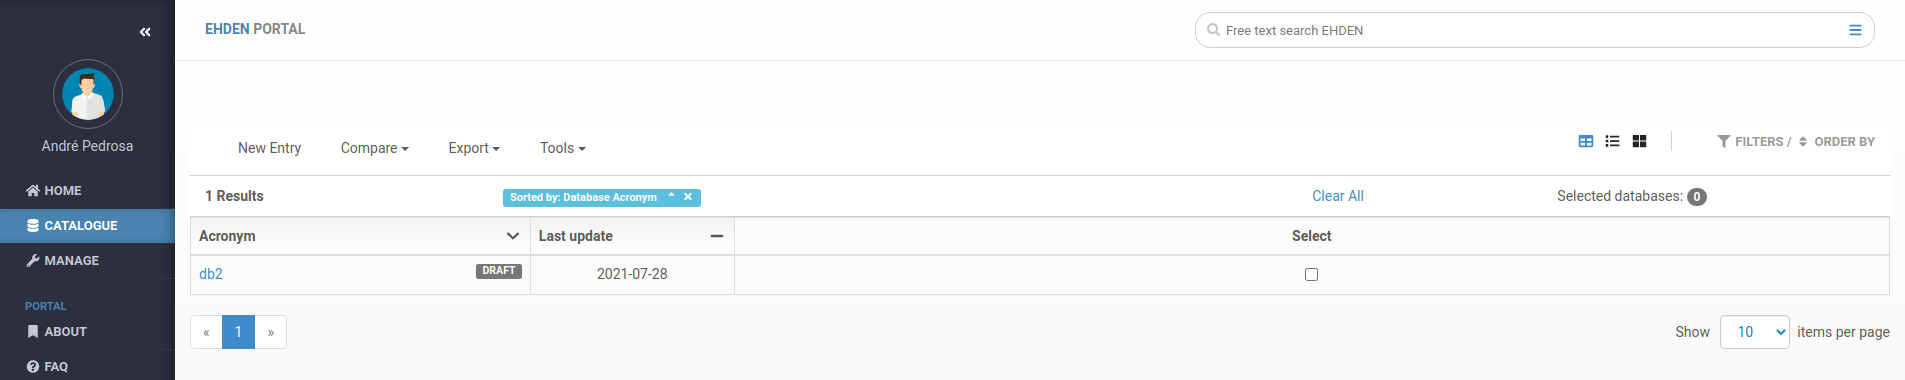
\includegraphics[width=\textwidth]{listings}
    \caption{The user interface displayed after selecting a community, which shows the list of the fingerprints of the chosen community.}
    \label{fig:listings}
\end{figure}

\subsection*{Views}

In figure \ref{fig:fingerprint-new} it is presented the user interface where a data owner can answer the questions of a questionnaire.
Each question of the questionnaire is placed under a container that can be collapsed, as is shown for the question \textit{Instituition name}.
However, if multiple questions are grouped, the collapsable container will affect all questions of the group.

\begin{figure}[H]
    \center
    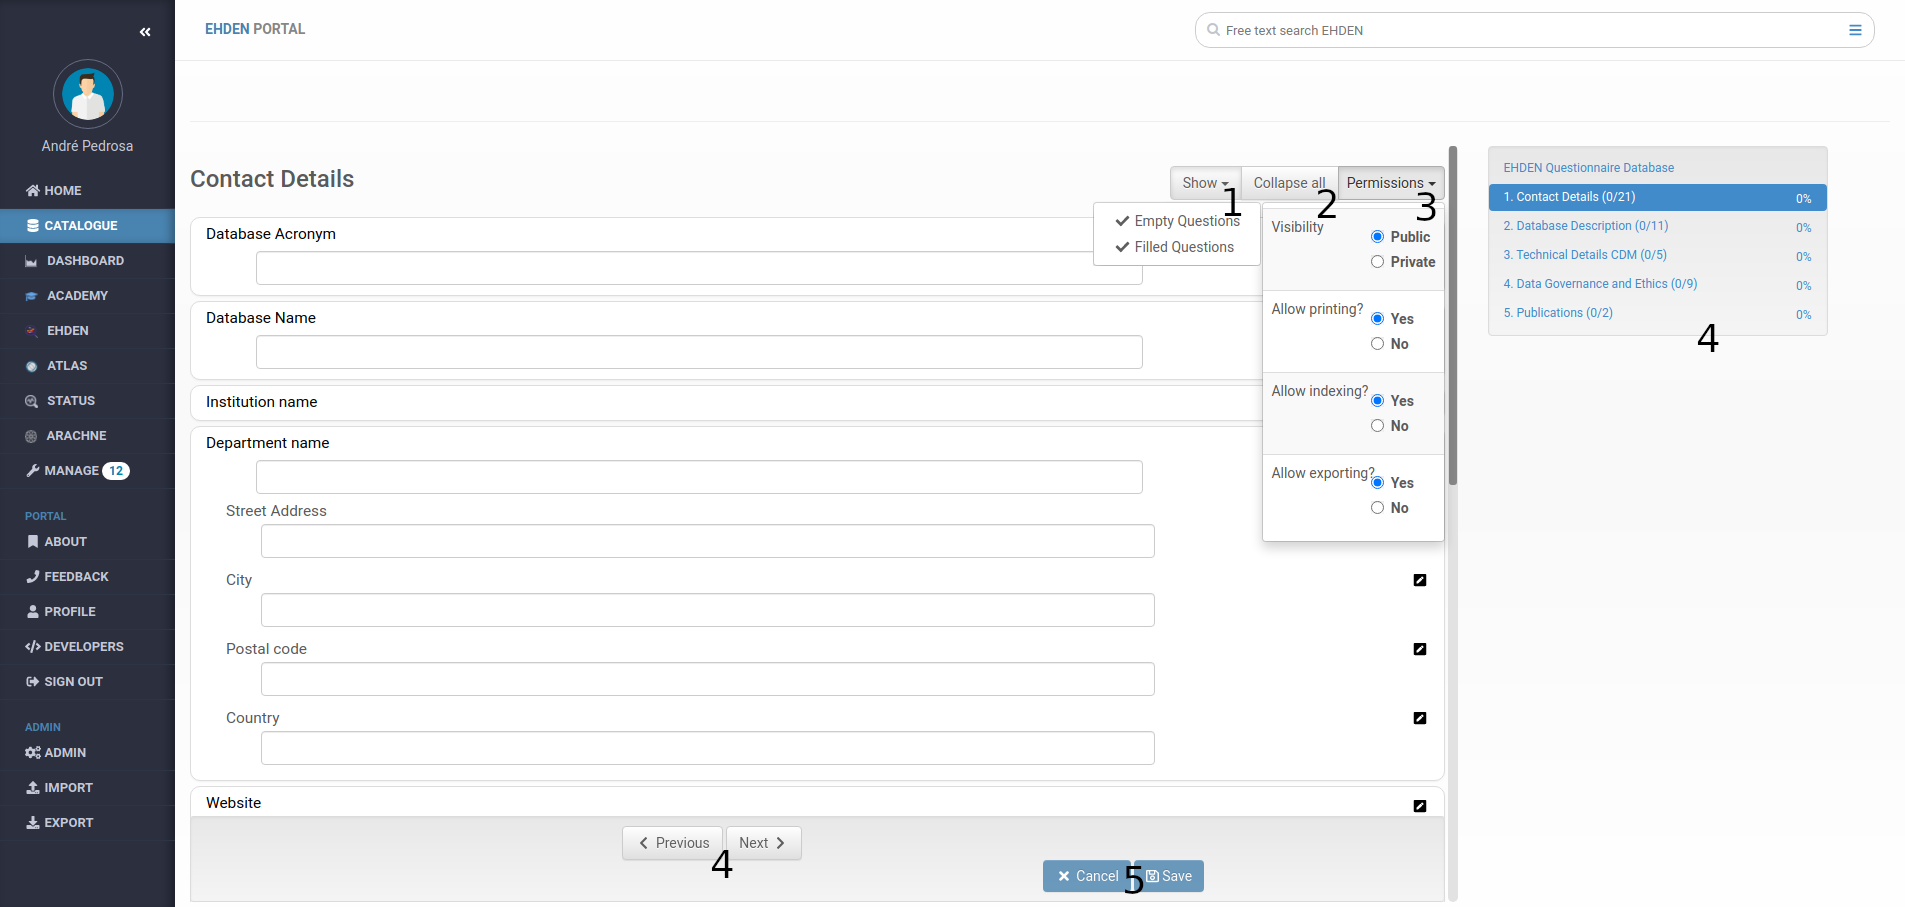
\includegraphics[width=\textwidth]{fingerprint-new}
    \caption{User interface to create a fingerprint.}
    \label{fig:fingerprint-new}
\end{figure}

Besides the input widget where the data owner can insert its answers, the user also has some additional control buttons:

\begin{enumerate}
    \item Allows to Hide or Show Questions that have been answered or that are empty. Besides being an interesting feature is important to note that on the last version it does not work, as clicking on the presented options will result in no visual effect;
    \item Allows to collapse or expand all questions or question groups containers;
    \item Allows the data owners to set permissions at the question set level;
        \begin{itemize}
            \item Visibility: Let plugins have access to answers data;
            \item Allow printing: On the fingerprints list page, showed in figure \ref{fig:listings}, there is a dropdown with tools, being the only one the "Print" tool (figure \ref{fig:listings-tools}). However, this feature is not correctly implemented since it calls the browser's built-int printing function on the fingerprint list page, so no actual fingerprint data will be printed. This permission ends up being useless. Additionally, if a user calls the browser's print function (e.g. hitting Ctrl+P) when viewing the data of a fingerprint, the platform will not block the action;
                \begin{figure}[H]
                    \center
                    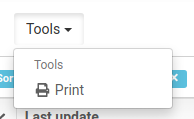
\includegraphics[width=.2\linewidth]{listings-tools}
                    \caption{Available tools on the fingerprint selection.}
                    \label{fig:listings-tools}
                \end{figure}
            \item Allow indexing: If the data owner allows indexing of the answers, which will allow for other users to find fingerprints based on the answers to a question of this specific question set;
            \item Allow exporting: If the answers to this question set can be included on the export file of a fingerprint.
        \end{itemize}
    \item Enable navigation along the question sets of the current questionnaire;
    \item Permits to save or cancel all the changes made to the current question set.
\end{enumerate}

Once the fingerprint is filled and published, a regular user can consult the metadata, which will be displayed by default in detailed view (figure \ref{fig:fingerprint-show-detailed}).
Similar to the create view, it is presented with some control buttons:

\begin{enumerate}
    \item Database level plugins associated with this community;
    \item Statistics of this fingerprint:
        \begin{itemize}
            \item Progress bar + Filled: How many questions of the questionnaire were answered;
            \item Hits: Number of times this fingerprint showed up on search queries;
            \item Unique Views: Number of users that visited this fingerprint.
        \end{itemize}
    \item Question set controls:
        \begin{itemize}
            \item Summary: Allows to switch to the summary view (Figure \ref{fig:fingerprint-show-summary});
            \item Collapse \& Show: The same role as mentioned for the create view.
        \end{itemize}
    \item Fingerprint control buttons:
        \begin{itemize}
            \item Subscribe: Receive notifications whenever changes are made to the fingerprint answers;
            \item Manage: Several fingerprint operations:
                \begin{itemize}
                    \item Edit: Enter the edit mode;
                    \item Share: Allows to add other users as owners of the fingerprint and also to create links that enable anonymous users to consult the fingerprint;
                    \item Export: Different forms of export. CSV, PDF, and MONTRA format to import on other installations of the MONTRA framework;
                    \item Delete: Remove the fingerprint from the community.
                \end{itemize}
        \end{itemize}
\end{enumerate}

\begin{figure}[H]
    \center
    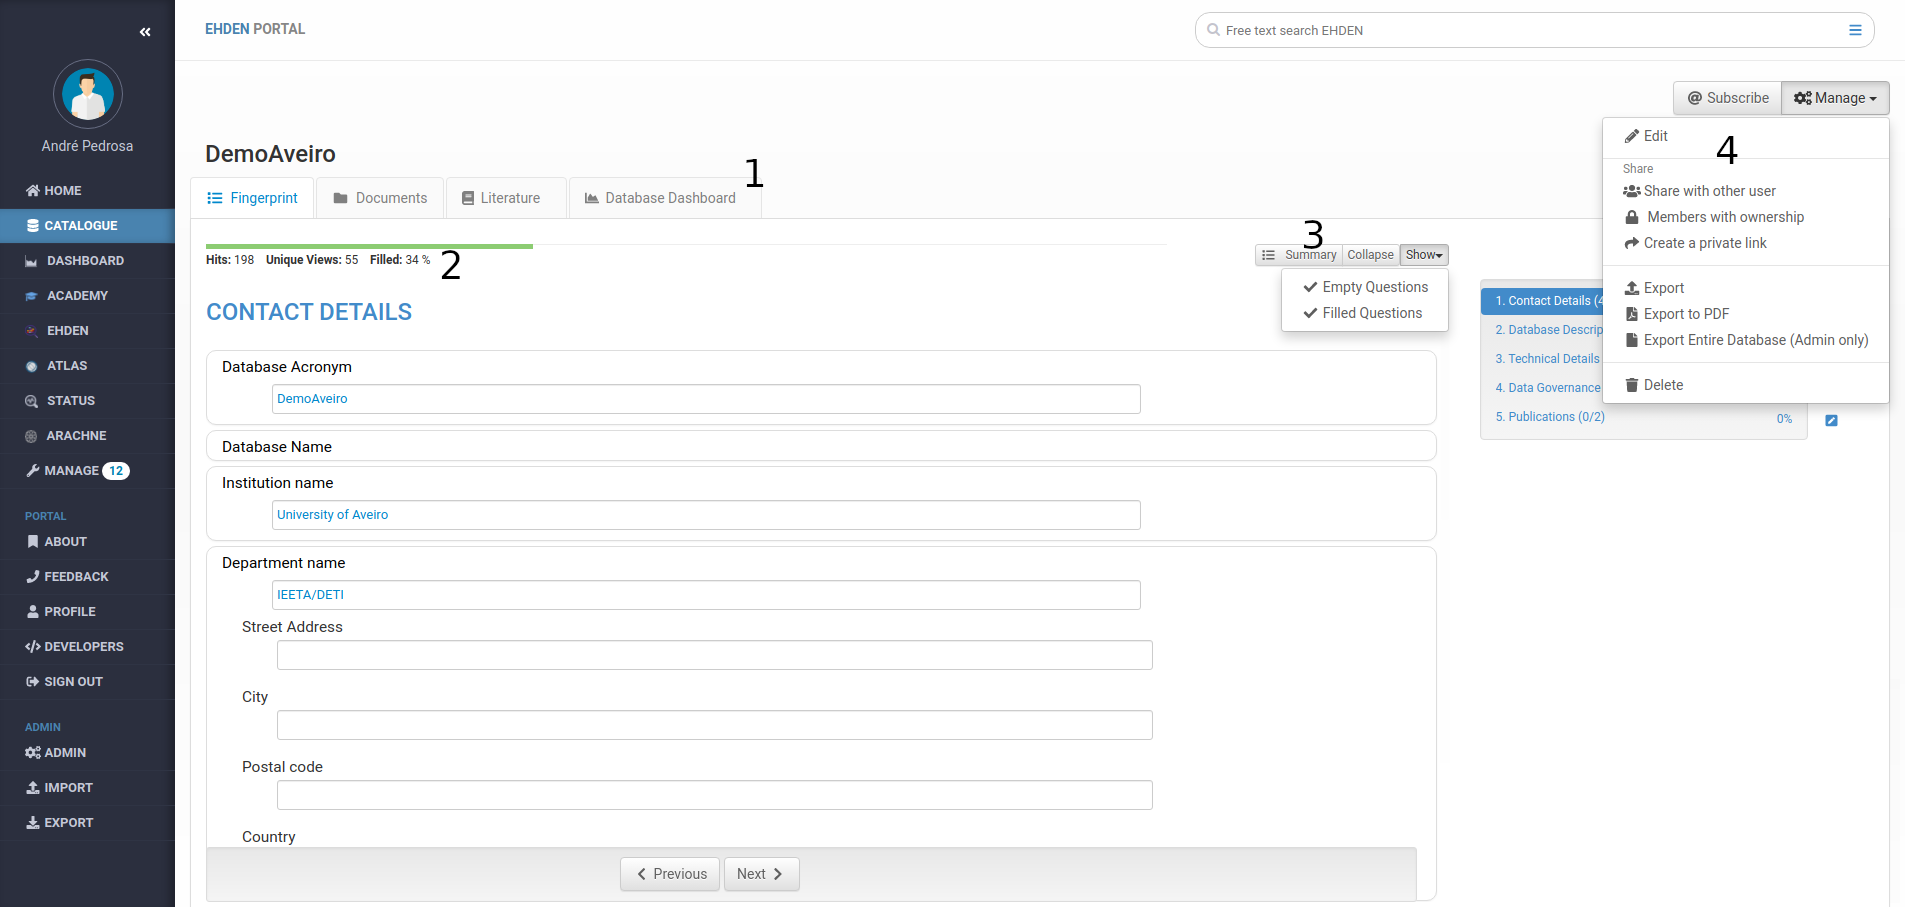
\includegraphics[width=\textwidth]{fingerprint-show-detailed}
    \caption{The detailed version of the interface to view and analyze fingerprints.}
    \label{fig:fingerprint-show-detailed}
\end{figure}

On the show view, if the user enters the summary view (Figure \ref{fig:fingerprint-show-summary}), the user is presented with a table with three columns where each row contains the question number, name and the answer given.
On this view, by hovering over an empty answer container the user can send a request to the database owner to answer the specific question.

\begin{figure}
    \center
    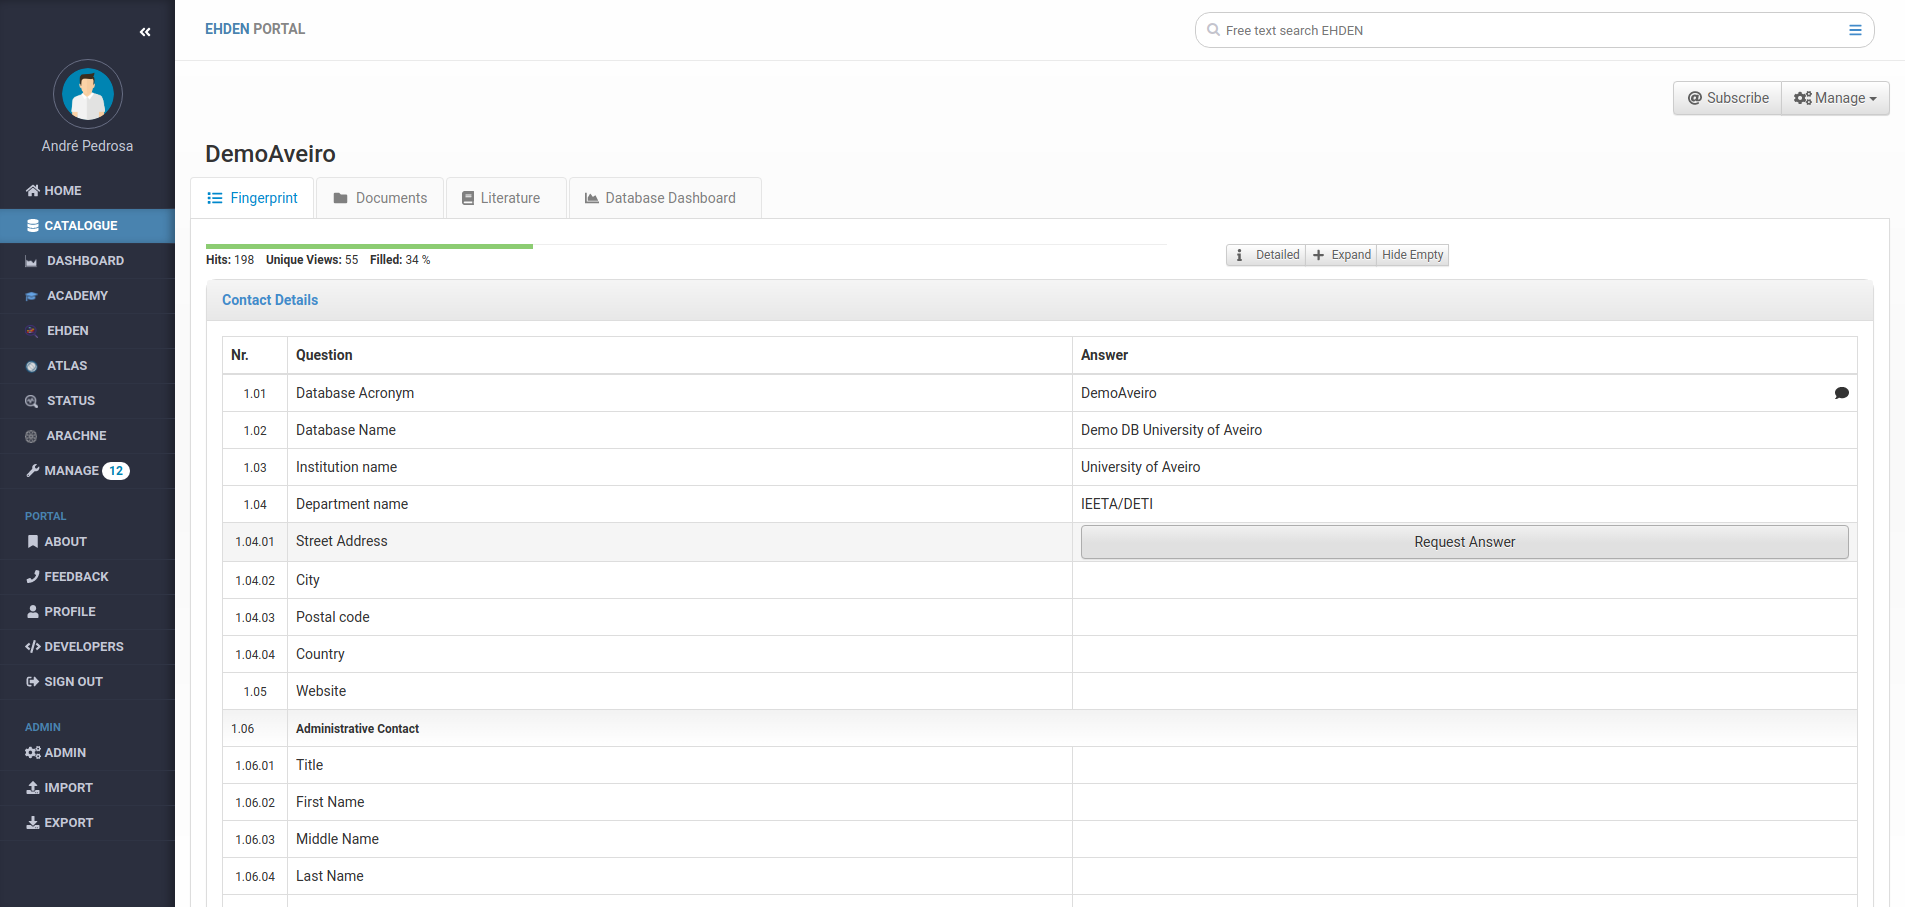
\includegraphics[width=\textwidth]{fingerprint-show-summary}
    \caption{The summary version of the interface to view and analyze fingerprints.}
    \label{fig:fingerprint-show-summary}
\end{figure}

The MONTRA framework also offers an ``Advanced Search'' feature, allowing to perform searches for fingerprints.
The overall interface used is identical to the ones presented above, where the user answers the questions of the specific questionnaire of the community.
The main difference to the other versions of the fingerprint view is that the only control buttons available are just the navigation ones, and all the questions do not have any validation.
Additionally, at the bottom of the page, it is provided to the user a way to customize the search query, allowing to create complex search criteria through a drag and drop interface, as is presented in figure \ref{fig:boolean-query}.

\begin{figure}[H]
    \center
    
\includegraphics[width=\textwidth]{boolean-query}
    \caption{Interface to customize the search query.}
    \label{fig:boolean-query}
\end{figure}

% ---

Despite all these variations of the same view having a similar look, as some components appear on several variants, all views have a separate Django template, so there is some duplicated code across the different views.
If some changes are made to a shared component, such as the side question set menu bar, those changes have to be applied to all different templates.
This can be avoided since the Django template system allows to both include a shared component into other templates and also supports conditional rendering, for example, the permissions dropdown for a question set of a fingerprint should only be rendered when the user is editing or creating a fingerprint.

% ---

These different view versions provide a valid workflow to perform \gls{crud} operations over the metadata related to a data source, however, views that are used to insert or edit metadata of a fingerprint present several flaws related to how the inputs are validated and how they are presented to the user.

First, the validation of the user input is done on the client-side through javascript code that runs after a user submits a question set form.
Subsequently, the data is sent to the backend through \gls{api} calls.
However, if one would use the \gls{api} directly to update metadata of the fingerprint, the validation could be skipped and invalid data could be stored on the database.
In some cases there might exist some validation code on the server-side, however, this brings the necessity to maintain two separate code files.

Second, there is no escaping procedure done to the user's input when it is fetched from the database which allows that \gls{xss} attacks can be easily performed and put users that consult a compromised fingerprint at risk.
As an example, on figure \ref{fig:montra-xss-create} on the Database Name field, I added a \textit{script} tag with code that shows a popup and also a valid database name after.
Once a user opens the fingerprint to check the data, the code will execute, but the dummy name will render on the Database Name field, as seen in figure \ref{fig:montra-xss}.
This can be further exploited, where the user visiting the fingerprint will not notice that malicious code was executed.

\begin{figure}[H]
    \center
    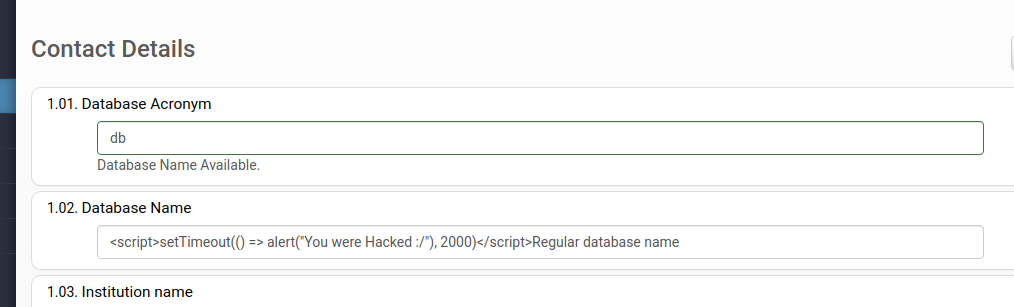
\includegraphics[width=0.75\textwidth]{montra-xss-create}
    \caption{Example of how an \gls{xss} attack could be done on MONTRA.}
    \label{fig:montra-xss-create}
\end{figure}

\begin{figure}[H]
    \center
    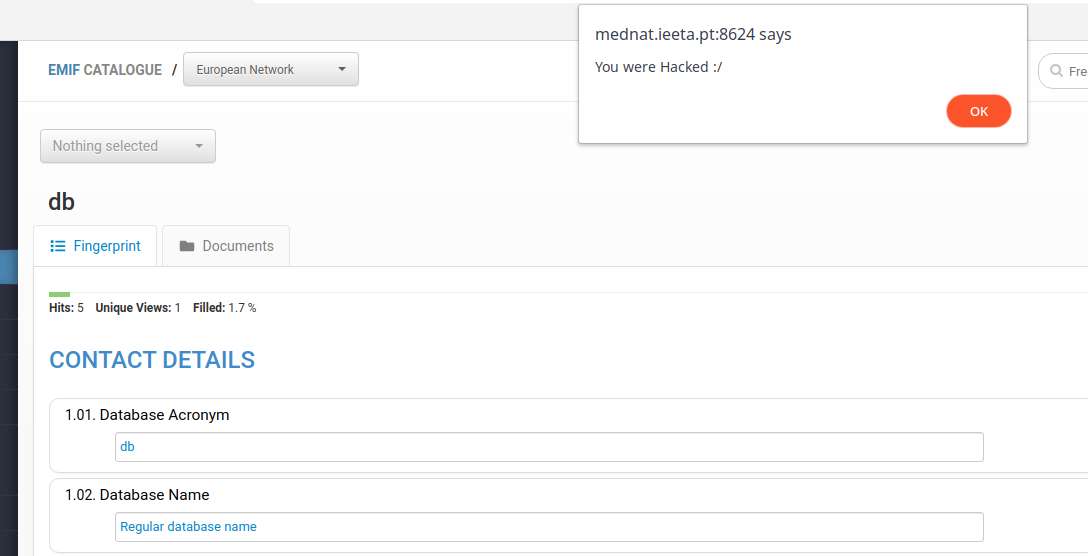
\includegraphics[width=0.75\textwidth]{montra-xss}
    \caption{Victim of a simple \gls{xss} attack.}
    \label{fig:montra-xss}
\end{figure}

All these problems exist because such views were developed from scratch without using the provided features that Django has out of the box for form validation and security.
For client-side validation, Django takes advantage of HTML5 form validation features~\cite{form-validation}.
This allows imposing restrictions and validations on the user's input without writing any additional javascript code.

To show these features I wrote a simple HTML file with a simple form that expects a number under 100 and an email.

\begin{verbatim}
<html>
  <body>
    <form>
      <label for"num">Number:</label>
      <input id="num" type="number" max="100">

      <label for"mail">Email:</label>
      <input id="mail" type="email">

      <button type="submit">Submit</button>
    </form>
  </body>
</html>
\end{verbatim}

If I try to submit the form with invalid values, error messages are presented as shown in figure \ref{fig:html-form-validation}.

\begin{figure}[H]
    \center
    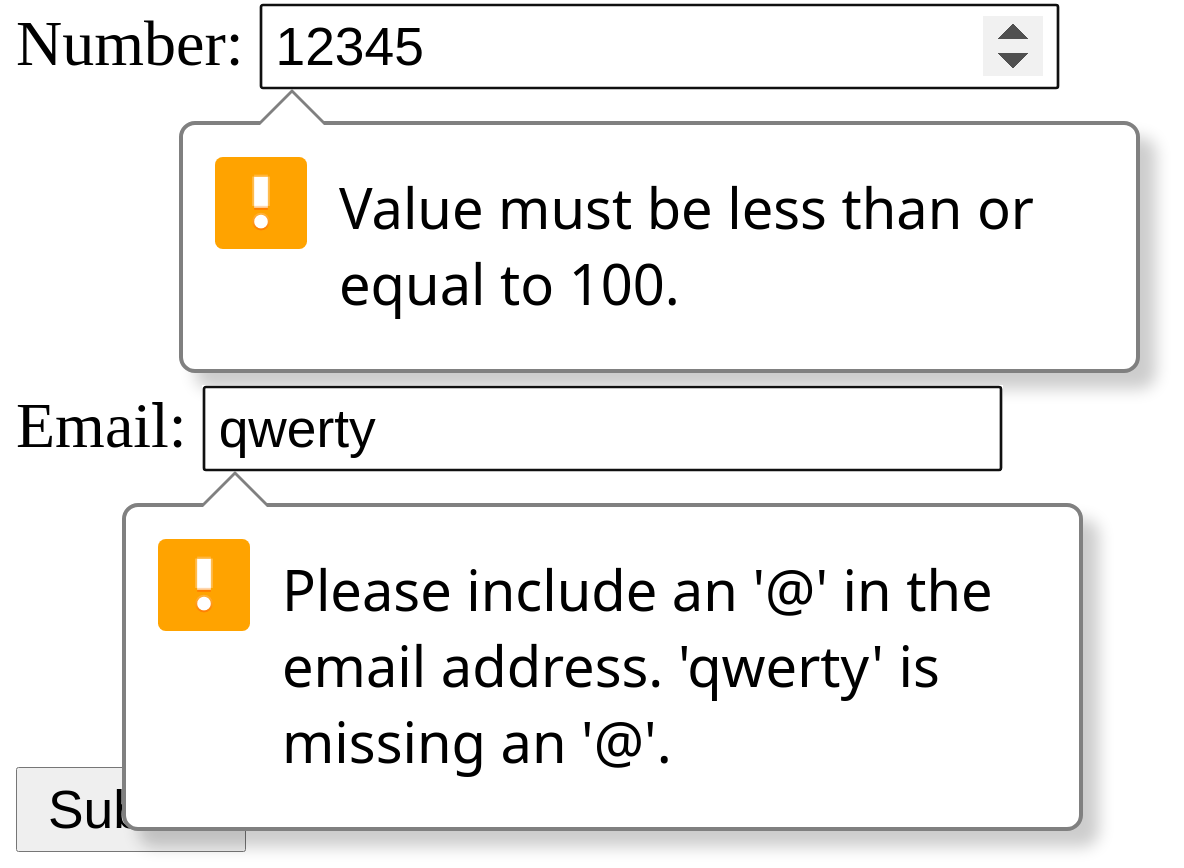
\includegraphics[width=.3\textwidth]{html-form-validation}
    \caption{Error messages that appear after submitting the form on a chromium based browser.}
    \label{fig:html-form-validation}
\end{figure}

Additionally, if the data is sent directly through an \gls{api} call to the backend, Django forms framework ensures that invalid data is rejected.
With this, when building a form in Django the developer only needs to specify what fields are present, their type and restrictions, and Django will validate all this before data is stored on the database.

Finally, \gls{xss} attacks are prevented because Django escapes the values that were previously provided by users when filling the input tags, e.g. the character ``<'' is transformed in ``\&lt;'', avoiding the browser to interpret user's input as \gls{html} code.

Another problem associated with the views of the MONTRA framework is how the management of javascript dependencies is done.
There is no consistency on how such dependencies are imported.
Some are imported directly on the template through \textit{script} tags making use of a \gls{cdn}, as others their entire source were added to the repository and are then referenced based on their location.
The first approach has the advantage that an upgrade is done by simply changing the URL attribute of the \textit{script} tag and also reduces bandwidth from the Django server handling the user requests.
The second approach increases the overall size of the repository, and the upgrade process will lead to more changes on the repository.
These processes, however, have the problem that easily unnecessary dependencies will still be present on the Django templates after being used on the application.
Currently, there are tools such as \gls{npm}\footnote{https://www.npmjs.com/} that help manage these dependencies by defining, on a single file, the dependency and its version.
This software will then download the dependency and subsequent dependencies.

\subsection*{Programming Interface}
% how submissions of fingerprint works

It was mentioned several times that some checks are not enforced through the \gls{api}.
It will be detailed now what calls are performed by MONTRA's fingerprint views.

Note that there are two different \gls{api}s available here.
Fingerprint views use one specific set of \gls{api} requests that return answers in \gls{html} format, ready to present to the user, and others to send the user's data.
For a regular user to use, there are other set o \gls{api} endpoints that are more human friendly, which are documented, and has a How to Use page, however, an advanced user can see what requests are made on the fingerprint views through browser's console and perform the requests themselves.

First, we will go over the \gls{api} used by the fingerprint views.
But before showing the available endpoints, let's go over how the fingerprint views are organized and how they show only the questions of a certain question set at a time.

Let use figure \ref{fig:fingerprint-hidden-question-sets} as example.
According to the right side menu, there are six question sets and currently the question set ``Contact Details'' is being presented.
In the middle of the page, we then see the content of the question set: questions, title, control buttons, and permissions.
Note that there is a scroll bar so the question set contains more questions.
Also the previous, next, cancel and save buttons are not tied to the question set.
The other question sets are also present on the page, however, they are hidden.
Every question set has its container, so whenever the user clicks on the previous or next buttons or selects another question set on the question set side menu bar, the current question set container is hidden and the new is shown.
For questionnaires with a high number of question sets, rendering all available question sets could not be necessary.
For that, a question set is only loaded when accessed the first time and following accesses will not require a load.

\begin{figure}[H]
    \center
    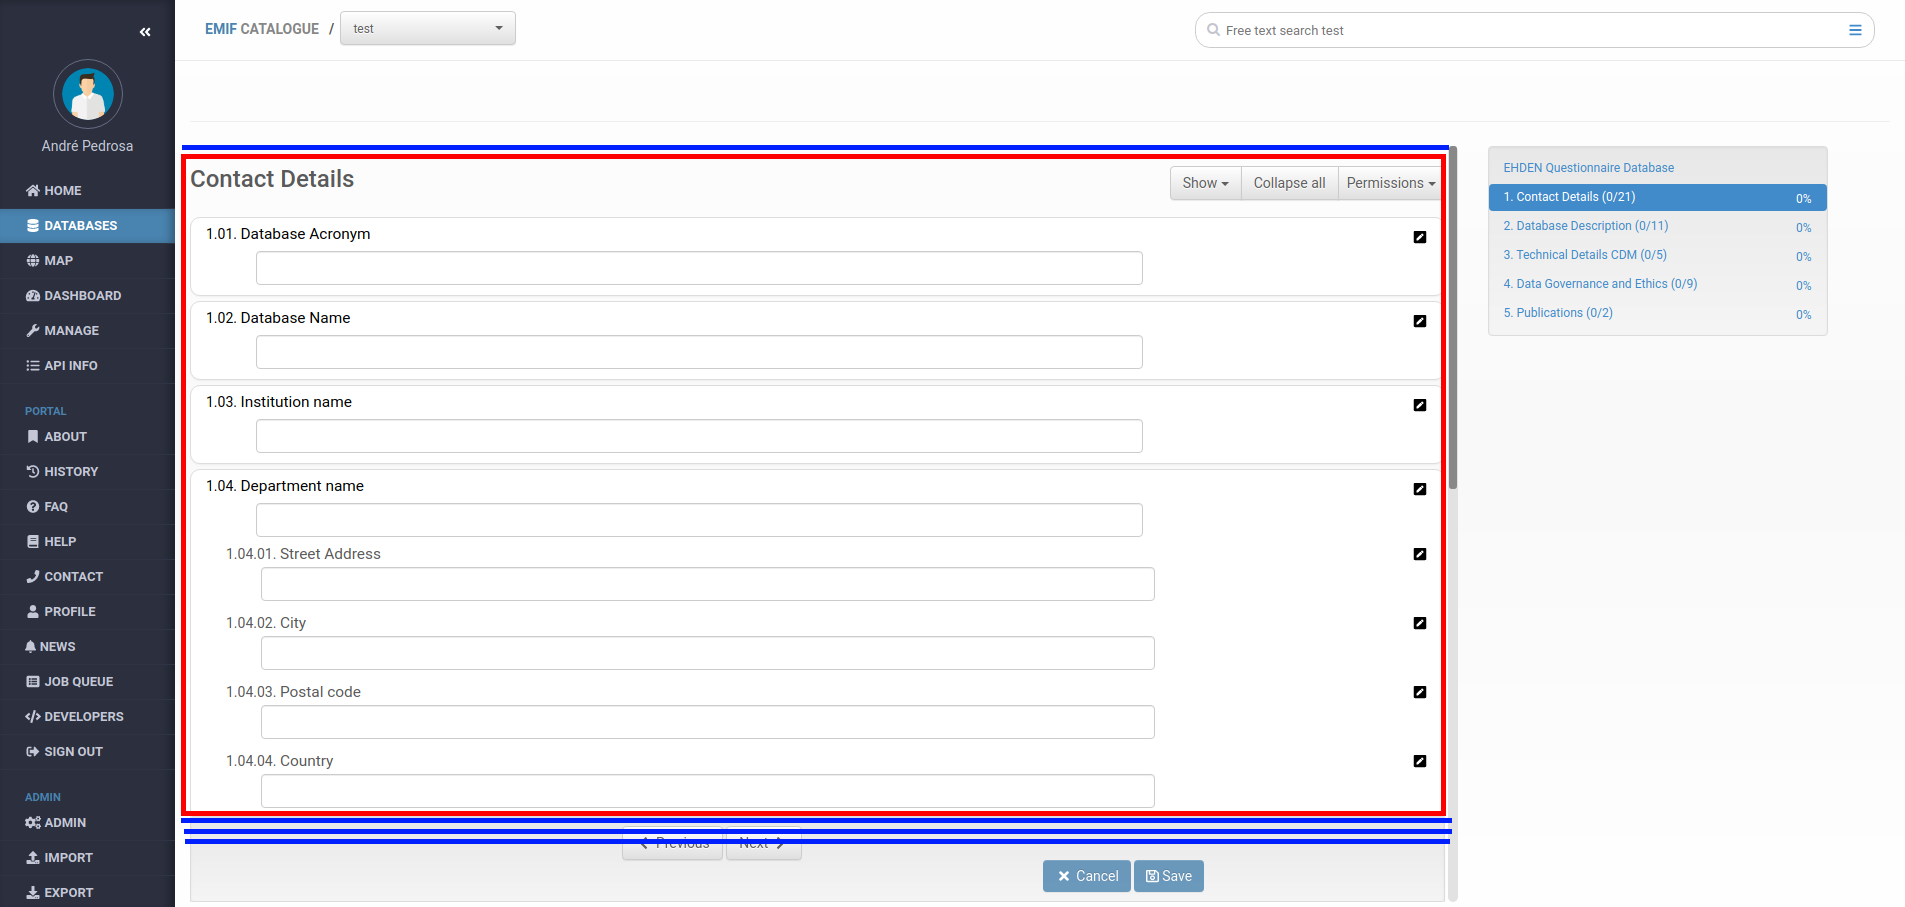
\includegraphics[width=\textwidth]{fingerprint-hidden-question-sets}
    \caption{Each question set has its container.
    Here the current container is presented within the red rectangle.
    The other existing question sets are represented through the blue lines, which are currently hidden.}
    \label{fig:fingerprint-hidden-question-sets}
\end{figure}

The fingerprint view can be used for four different use cases:
\begin{itemize}
    \item Create a new fingerprint: The questions are presented with clear and editable inputs;
    \item Edit an existing fingerprint: All questions are editable but the previously answered questions are filled;
    \item View the answers of a fingerprint: A read-only version of the fingerprint's answers;
    \item Search for fingerprints: Same as creating a new fingerprint, however, no validations are performed on the user's input.
\end{itemize}

For these use cases, the following endpoints are used:

\begin{itemize}
    \item Create:
\begin{lstlisting}[basicstyle=\tiny]
GET [base url]/c/[community slug]/addqs/[fingerprint hash]/[questionnaire id]/[question set id]/
POST [base url]/c/[community slug]/addPost/[questionnaire id]/[question set id]/[save id]
\end{lstlisting}
    \item Edit:
\begin{lstlisting}[basicstyle=\tiny]
GET [base url]/editqs/[fingerprint hash]/[questionnaire id]/[question set]/
POST [base url]/c/[community slug]/addPost/[questionnaire id]/[question set id]/[save id]
\end{lstlisting}
    \item View:
\begin{lstlisting}[basicstyle=\tiny]
GET [base url]/detailedqs/[fingerprint hash]/[questionnaire id]/[question set id]/
\end{lstlisting}
    \item Search:
\begin{lstlisting}[basicstyle=\tiny]
GET [base url]/c/[community slug]/searchqs/[questionnaire id]/[question set id]/
\end{lstlisting}
\end{itemize}

For both cases where new data is stored, besides the usual GET that is used to load the question set, there is also a POST request that saves the progress done to a specific question set.
The data for these requests are gathered natively by javascript since each question set container contains a \textit{form} tag englobing all the questions inputs.
This way there is no need to iterate over the questions of a question set and append each response to the request's data.
The \textit{save id} field of the endpoints tells to which question set the data is related to.
However, there is already a \textit{question set} field which always has the value of 1, so one of these fields could be removed from the endpoint.

The GET request is then used to load the \gls{html} to present the questions of a question set.
Note that the returned data is just the \gls{html} data to be placed on the respective question set container and not the whole fingerprint page.

Moving now to the set of \gls{api} endpoints available to the users to both read and update answer data the following are available:

\begin{verbatim}
GET /api/fingerprints/[fingerprint hash]/answers/
GET /api/fingerprints/[fingerprint hash]/answers/[question slug]
PUT /api/fingerprints/[fingerprint hash]/answers/[question slug]
\end{verbatim}

The first two GETs are used to retrieve answers data, which is returned as the \gls{json} object presented next, the only difference being the first one returns an array of the mentioned object instead of just one.

\begin{verbatim}
{
  "question":"patients_count",
  "data":""
}
\end{verbatim}

With the PUT request, a fingerprint owner can update data of specific answers where a \gls{json} object should be sent in the body of the request with the field ``data''.

\begin{verbatim}
{
  "data": 10000
}
\end{verbatim}

Existing two different types of endpoints to retrieve answers data makes sense since the returned format is returned in a way that is easier to handle data by the target entity that will consume that endpoint.
If the fingerprint pages receive the data in \gls{html} format they can just put the \gls{html} in the determined container instead of having to build the entire container and insert the data on each input.
Accordingly, if data is returned in a \gls{json} format, data can be easily accessed, avoiding having to transverse the \gls{html} and retrieve the data from each input.
However, having two different endpoints to update data does not make that much sense since current \gls{http} requests libraries offer an easy way to build a request in the required format as the one's browsers automatically build whenever a form is submitted.

\subsection*{Draft Status Changes}

We will also go over the \gls{api} endpoints that the front end code uses to request to change the fingerprint state from draft to published.
Associated with this feature, there are two endpoints available:

\begin{verbatim}
POST [base url]/api/pending/[fingerprint hash]
POST [base url]/api/draft/[fingerprint hash]
\end{verbatim}

The existence of two endpoints for the same purpose is because Communities have a setting that allows to auto-accept requests to publish a fingerprint.
For that, whenever the auto-accept setting is off, the first endpoint must be used, which will send a request to the community owners to publish the given fingerprint.
The second must be used otherwise.

The problem with this approach is that the code that decides what endpoint to use is on the client-side and there is no server-side check if the correct endpoint is being used.
If the auto-accept setting is off and the second endpoint is used, a user can publish his fingerprint without requiring the approval of the community owners.

\subsection{Import Questionnaires - Excel}
\label{subsection:excel}
% Como os vários conceitos anteriores são mapeados para o excel
% Question Sets
% Questions
% Choices
% ...

As mentioned before, to define a skeleton of the metadata that describes a data source for a given community, a spreadsheet file has to be submitted.
There is already a template with some instructions and columns where a community manager only has to fill the necessary rows to then get the wanted result.

The columns defined in the template are the following:
\begin{itemize}
    \item Type: the type of the specific row. Here are allowed 3 different values:
        \begin{itemize}
            \item QuestionSet: allows dividing the questionnaire into several sections;
            \item Question: a question specification;
            \item Category: allows to create a group of questions inside a question set.
        \end{itemize}
    \item Text/Question: label/name given to the item being defined;
    \item Level/Number: use as a level for questions and categories and number otherwise. As level allows to create groups of questions inside a question set. As number defines the number, and subsequently the order, of the question sets;
    \item Data type: used only for rows of type Question, specifying the question type;
    \item Value list: used to indicate extra information to build the question;
    \item Help text/Description: a small text that will be displayed along with the item being defined;
    \item Tooltip: Yes if the Help text/Description should be displayed as a tooltip or No otherwise;
    \item Slug: internal identifier;
    \item Dependencies: used to tell that a question or group of questions can only be answered if a specific choice of a choice-based question was selected;
    \item Stats, Comments Stats and Disposition: Columns that were used for old features but are still present on the spreadsheet;
    \item Include in Advanced Search: if the answers of the question can be used to search fingerprints.
\end{itemize}

\subsection*{Question Groups}
From the previous list, question groups were mentioned both when the type column has the Category value and on the Level part of the Level/Number column.
The former is used to add a title with no question associated, resulting in what is presented in figure \ref{fig:question-group-category}.

\begin{figure}[H]
    \center
    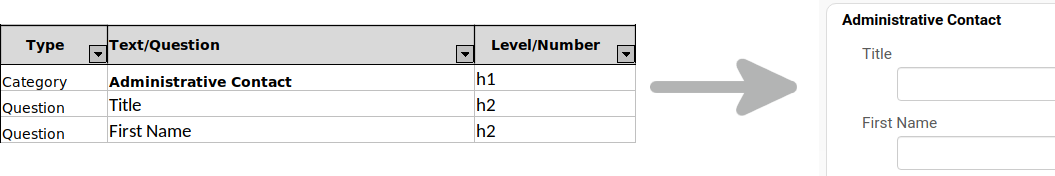
\includegraphics[width=\textwidth]{category}
    \caption{Create a group of questions with a title.}
    \label{fig:question-group-category}
\end{figure}

On the latter, the text of the question in the most upper level is used as the title of the questions group, resulting in an output similar to the one in figure \ref{fig:question-group-levels}.

\begin{figure}[H]
    \center
    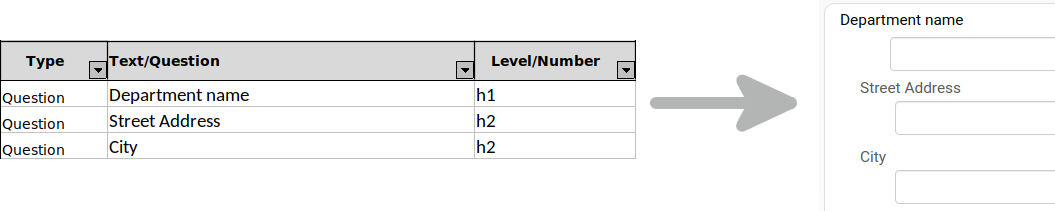
\includegraphics[width=\textwidth]{levels}
    \caption{Create a group of questions using a question's text as the title.}
    \label{fig:question-group-levels}
\end{figure}

It is important to highlight that the category way to create question groups is not independent of levels.
If both a category row and a question are on the most upper level, MONTRA will render two separate collapsable containers, where the first one will be empty, as is shown in figure \ref{fig:question-group-category-wrong-levels}.

\begin{figure}[H]
    \center
    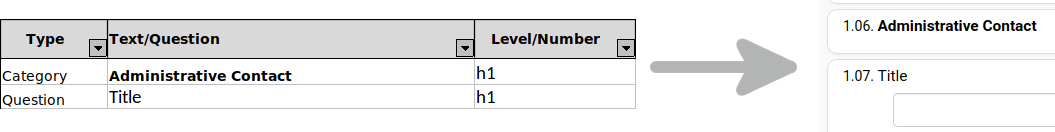
\includegraphics[width=\textwidth]{category-levels}
    \caption{Example to show that the category way to create question groups also depends on the values that are set on the level column.}
    \label{fig:question-group-category-wrong-levels}
\end{figure}

\subsection*{Value list}

To avoid having a spreadsheet with several columns that will not be used for all types of rows, the value list column expects some extra information required for some types of questions.

\subsubsection*{Choices}

For choice-based questions, the value list column is used to define the possible choices and to add an extra text field associated with a given choice.
Choices are separated by a ``|'' character and the extra text field can be set by appending ``\{...\}'' after the target choice's text.

\begin{figure}[H]
    \center
    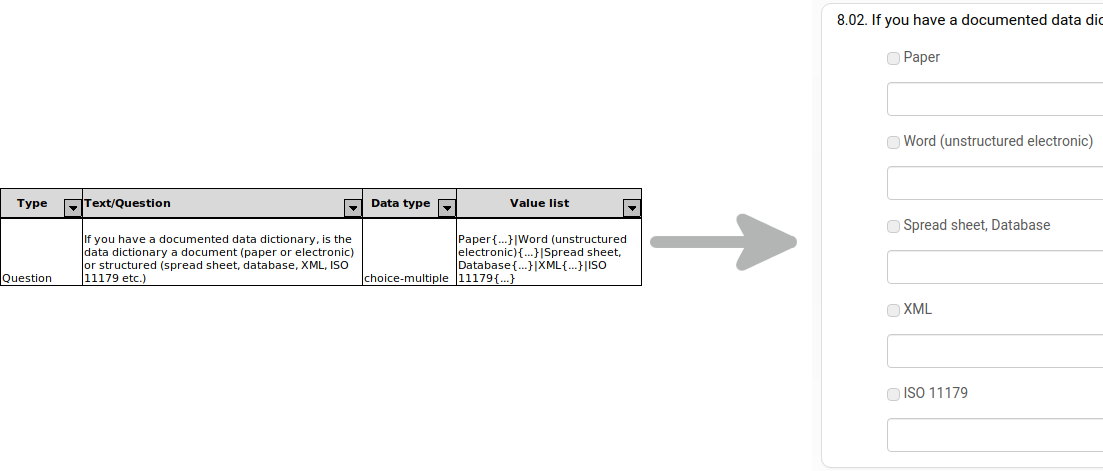
\includegraphics[width=\textwidth]{choice-freeforms}
    \caption{Multiple choice question with some extra text fields associated with the several choices.}
\end{figure}

Although the framework allows the extensibility to have an additional text field, these do not support other types of input and also have no validation.
Also, if the number of choices is high and the text is long, there starts to exist some clutter on the spreadsheet.
With this, the person creating the spreadsheet will have problems perform edits and check if there is something wrong or missing.

To facilitate the job of who is filling the spreadsheet, some question types are shortcuts.
For example, the choice-yesnodontknow is a question of type choice with three possible options: Yes, No, Do not Know.
Choice variants with freeform on the name, besides the usual choices, always have an additional text field, associated with the question instead of a choice.

\subsubsection*{Open Multiple Composition}

Open multiple questions allow showing a history of a given value.
For that the simple version of the question is represented in a table of two columns: Date and the value, so no input is expected on the value list column.
The composition version of the question type allows having several values, instead of just one.
In a way, the simpler version can be used as a shortcut question type, since it can be reproduced with the composition variant.

To render this question type, a third-party widget called Tabulator\footnote{http://tabulator.info/} is being used.
The configuration of such widget, expects an array of \gls{json} objects, each specifying some configuration of each column.
To configure the open multiple composition question type, the value list column expects these \gls{json} objects, where the date column is implicit.
The MONTRA framework will then put the provided objects on the configuration array that the Tabulator widgets expects, adding the configuration for the date column.

\begin{figure}[H]
    \center
    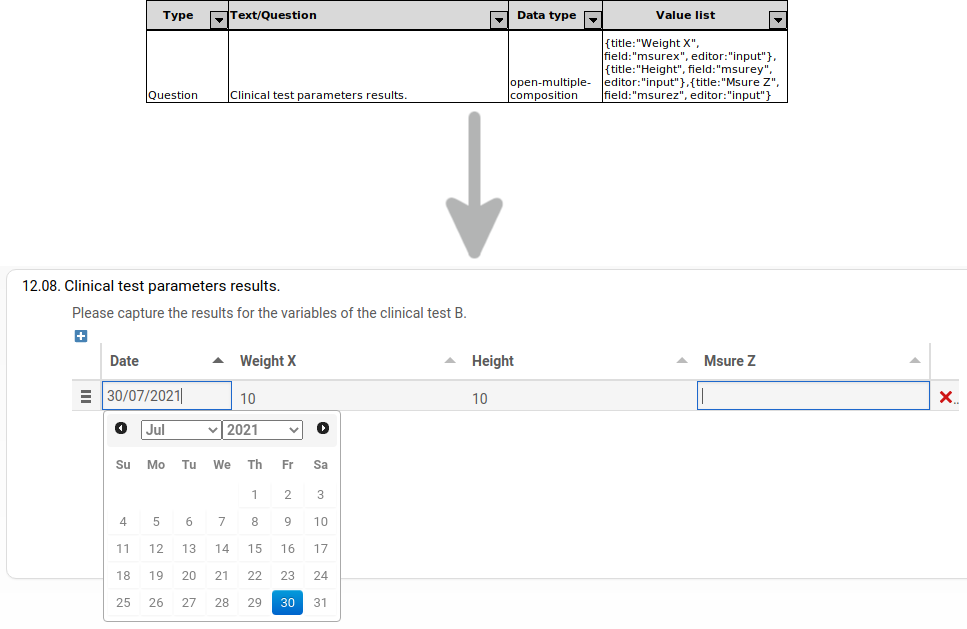
\includegraphics[width=\textwidth]{open-multiple}
    \caption{How an open-multiple-composition question type is specified on the spreadsheet and how it is rendered.}
    \label{fig:open-multiple}
\end{figure}

\subsubsection*{Choice Tabular}

This type of question allows reusing the same choices across several answering items.
There are three variations of this questions types, where the difference between them is what and how is the information connected between answering items and choices.
There are two versions where the user can select one (single choice) or more (multiple-choice) choices for each answering item.
The other version allows the user to write text for each choice within each answering item.
The question type is rendered as a table where in the columns are displayed the several choices and on the rows the different answering items are presented.
Additionally, there can be a ``More'' choice column, where the user can insert any text information for a specific answering item since is displayed with a textarea \gls{html} element.

The value list column of a choice tabular question type expects a three-component value.
Each component is separated by the characters ``\textbackslash\textbackslash''.
Within each component, items are separated by the ``|'' character.
The components are the following:

\begin{itemize}
    \item choices (columns);
    \item answering items (rows);
    \item type of the information: available values are choice, multiple-choice and text.
\end{itemize}

Once again, we encounter the clutter problem, as shown in the spreadsheet section of figure \ref{fig:choice-tabular}, which hampers readability and update of the value list field.

\begin{figure}[H]
    \center
    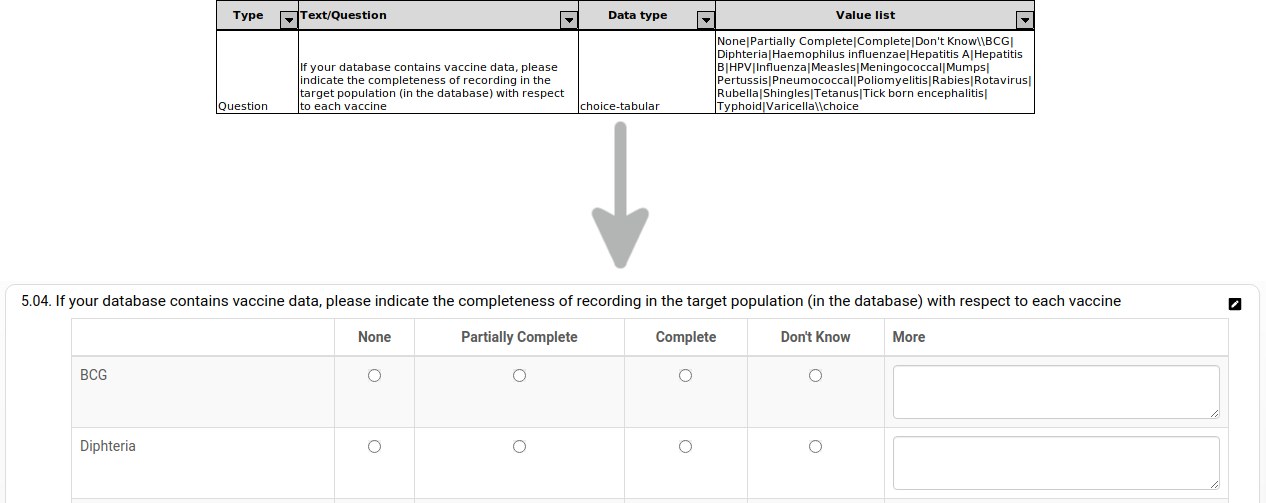
\includegraphics[width=\textwidth]{choice-tabular}
    \caption{How a tabular-choice question type is specified on the spreadsheet and how it is rendered.}
    \label{fig:choice-tabular}
\end{figure}

\subsection*{Dependencies}

In several form applications, it is common to find situations where if a certain choice is selected, then other questions will show up.
E.g. If a user answers ``Yes'' to the Question ``Have you visited Aveiro?'', then other questions such as ``Would you recommend it to a friend?'' would appear.

MONTRA supports this kind of dependencies, which should be defined on the Dependencies column of the questionnaire spreadsheet.

\begin{figure}[H]
    \center
    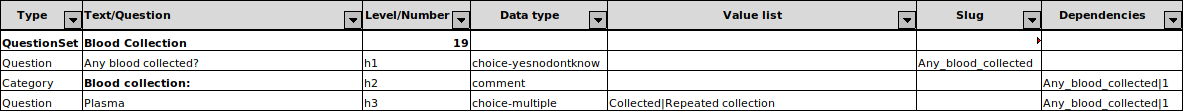
\includegraphics[width=\linewidth]{dependencies-excel}
    \caption{An example of both a question and a category that depend on the selected value for another question.}
    \label{fig:dependencies-excel}
\end{figure}

As shown in figure \ref{fig:dependencies-excel}, first you should indicate the slug of the question on which the specific question depends.
Then, separated by a ``|'' character, it must be specified which choice has to be selected for the dependency to be fulfilled, using its index, starting at 1.
On figure \ref{fig:dependencies-excel}, since a choice-yesnodontknow question type has three implicit choices, by having a dependency with the value ``Any\_blood\_collected|1'', both the \textit{Blood collection} category and the \textit{Plasma} question will only be displayed to the user once the choice \textit{Yes} of the \textit{Any Blood Collection?} question is selected.

\begin{figure}[H]
    \center
    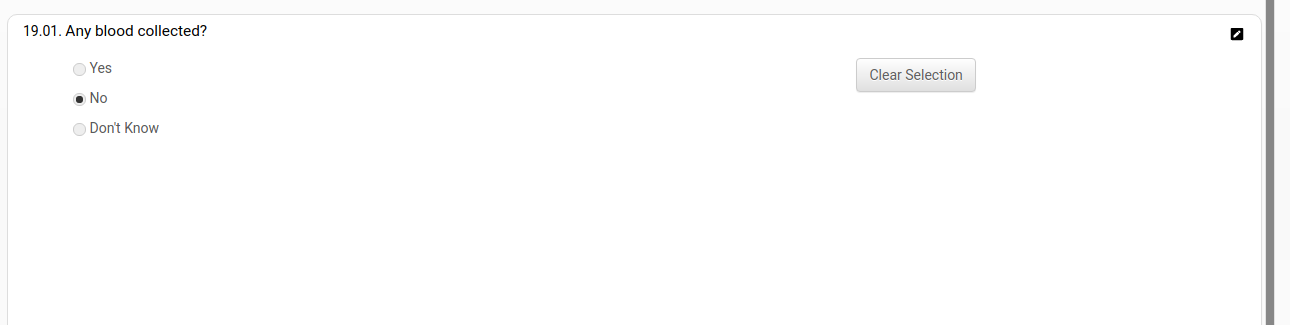
\includegraphics[width=0.75\linewidth]{dependencies-no}
    \caption{The questions with dependencies are not rendered if the specific choice is not selected.}
    \label{fig:dependencies-no}
\end{figure}

\begin{figure}[H]
    \center
    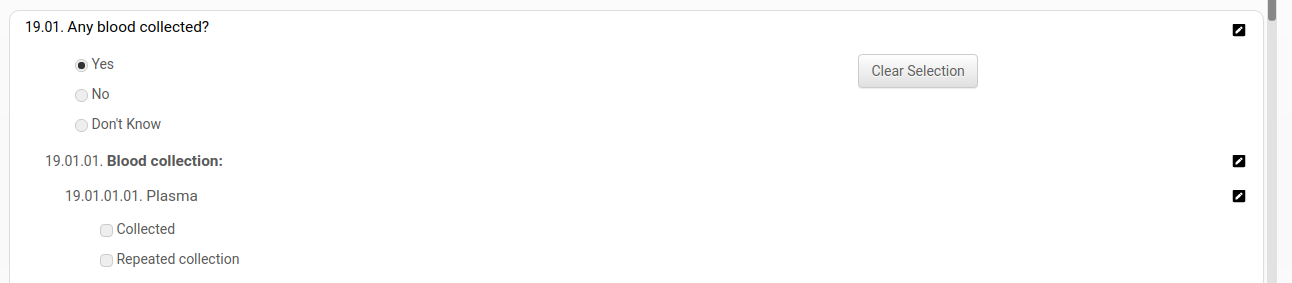
\includegraphics[width=0.75\linewidth]{dependencies-yes}
    \caption{Once the dependency of a specific question is meet it will be rendered.}
    \label{fig:dependencies-yes}
\end{figure}

Besides such restrictions are imposed on the user when he visits the web page, if the API was used directly, such dependencies would not be checked, which would lead to unnecessary data be stored on the database since it will not be displayed to the user.

\subsection{Data Models}
% Diagrama de classes
% Principal intuito de cada class
% answers (todos os tipos guardados em texto)

This section will present how the previous concepts are mapped to database models.
Taking advantage of Django's \gls{orm} feature, MONTRA's data models are defined as python classes that extend Django's base Model class.
These Model classes belong to different applications, which are associated with distinct aspects of the platform.

In figure \ref{fig:old-models} is presented the class diagram of the classes that are related to features and/or concepts that were mentioned in previous sections.
Classes with the same color belong to the same Django application, dividing them into specific purposes.

\begin{figure}[H]
    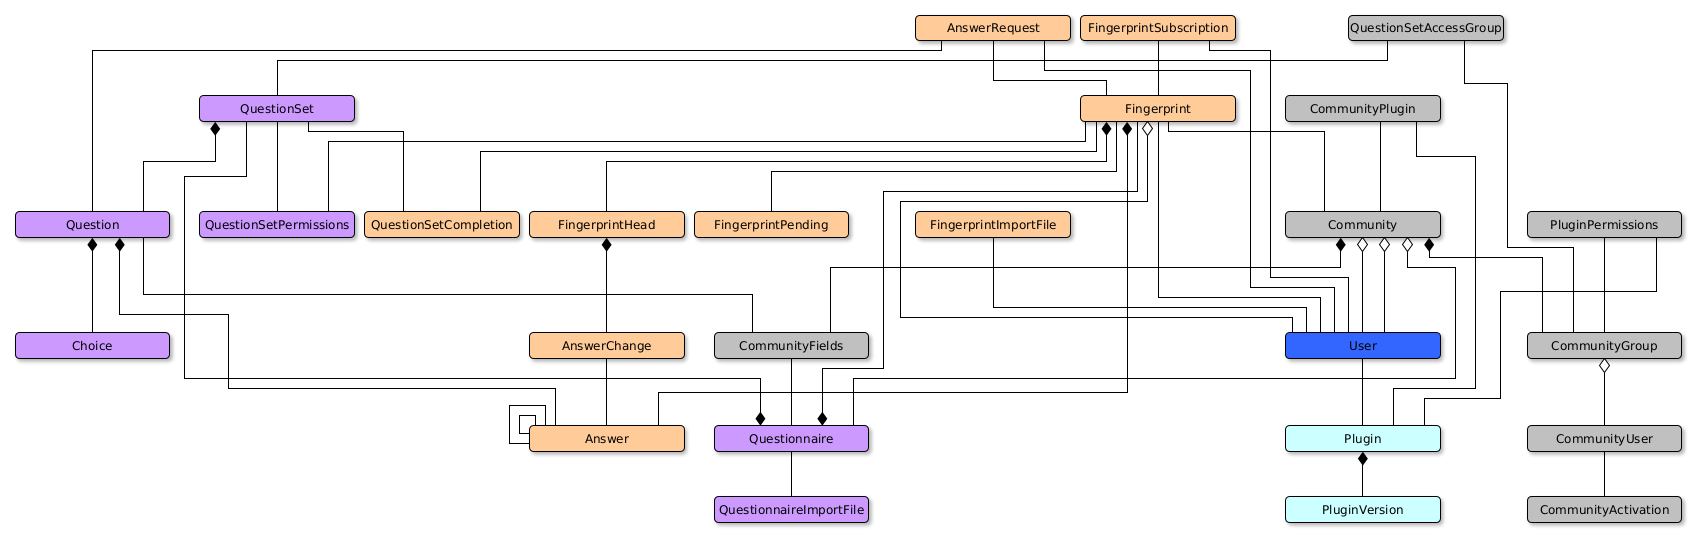
\includegraphics[width=\textwidth]{old-models}
    \caption{Class diagram of MONTRA's Model classes. Each color has a Django application associated. Gray: Community; Purple: Questionnaire; Orange: Fingerprint; Light Blue: Plugin; Blue: Django Auth. MONTRA's data model is much more complex, however, it is just presented the ones that impact the features and/or concepts mentioned previously.}
    \label{fig:old-models}
\end{figure}

\begin{itemize}
    \item Blue - Django's built-in authentication system\footnote{https://docs.djangoproject.com/en/1.11/ref/contrib/auth/};
    \item Orange - Fingerprint application: Answers to questionnaires questions and other models associated with features that were mentioned on the fingerprint views section, such as AnswerRequest and FingerprintSubscription.
        MONTRA also keeps a record of all the states of a given Fingerprint.
        For that, it uses the FingerprintHead model, which maps to a set of AnswerChanges;
    \item Purple - Questionnaire application: Questionnaires structure information such as question sets, questions, and choices, and import spreadsheets logs. Additionally, associated with each fingerprint, contains a model with the allowed permissions on each question set;
    \item Light Blue - Developer application: Allows adding customizations to different MONTRA's installations through plugins;
    \item Gray - Community application: Community's groups, users and access permissions, fields to be presented on the fingerprint list page for each questionnaire and plugins.
\end{itemize}

% ---

Going into more detail on some models we can see some poor design decisions.

Regarding fingerprint answers to a questionnaire, all the data is stored in the Answer model on the data field, which is a variable-length string field type.

\begin{figure}[H]
    \center
    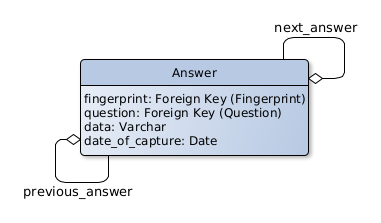
\includegraphics[width=.4\linewidth]{answer-model}
    \caption{Detailed information of the Answer model of the Fingerprint application.}
    \label{fig:answer-model}
\end{figure}

Although this approach is much simpler in terms of data models, it leads to two problems:
\begin{enumerate}
    \item this is not the most optimized way to store all the data types.
        Some question types expect numeric values and other date values, which could use built-in field types of a \gls{rdbms};
    \item for complex question types which the answer contains several fields, before and after storing such data in the database, some processing has to be made to convert the data to the necessary format.
        One example of this is multiple choice questions, where the value of the several selected choice is joined in a single string to then be stored on the database.
        Every time the answer needs to be displayed to a user, it is necessary to split that string by its separator.
        For this situation instead of storing the choice's value, the models of the questionnaire application could be used as a foreign key.
\end{enumerate}

Related to MONTRA itself, when a user provides no data to a specific question, an empty string will still be sent for that question on the submission of the answers to a question set, which will create unnecessary records on the database.

As mentioned previously, MONTRA records the history of submissions for a specific fingerprint.
Each submission has an associated FingerprintHead record, which its name might have been inspired by the HEAD concept of Git\footnote{https://git-scm.com/}, a version control system.
For every FingerprintHead there is a set of answers that suffer changes which are then recorded on the AnswerChange model.
In this model, we can get the answers data duplicated three times since it is already stored on the Answer model and can also be stored again as text in both \textit{old\_value} and \textit{new\_value}.

\begin{figure}[H]
    \center
    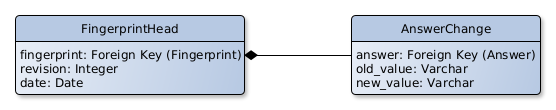
\includegraphics[width=.6\linewidth]{answer-changes-models}
    \caption{Models that store the changes to answers of fingerprint.}
    \label{fig:answer-changes-models}
\end{figure}

% ---

As mentioned previously, a fingerprint is not immediately available to all regular users, since it first enters on a draft state.
To transit to the published state, a request needs to be made to the community owner.
Such requests are stored on the FingerprintPending table, where the pending value will be \textit{true}.
Once a request is rejected or accepted, the value of the pending value is changed to \textit{false}.

\begin{figure}[H]
    \center
    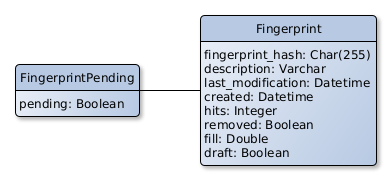
\includegraphics[width=.6\linewidth]{fingerprint-pending-models}
    \caption{The Model that stores the information telling if a fingerprint is waiting to be approved to be published.}
    \label{fig:fingerprint-pending-model}
\end{figure}

On the Fingerprint model, there is also a \textit{draft} value that indicates if the fingerprint is published or not.
Once a fingerprint is published, the value of the \textit{draft} will be true, and on the FingerprintPending table, the associated record will have the pending value at \textit{false}.
However, this value is not required to be stored on the database since after a fingerprint is published, the fingerprint will not be pending, therefore, the associated FingerprintPending record could be deleted.

% ---

Whenever a questionnaire is imported, a QuestionnaireImportFile record is created containing the information of the uploaded file and the user that uploaded it.
Also contains a status field to give some feedback to the user.
Associated with every import, it will also be created a Questionnaire record.
It contains an in\_preview variable that is set to \textit{true} whenever a questionnaire is in the import process.
If it fails to import, only the QuestionnaireImportFile record will be kept, which the status will change to \textit{Failed} and an error message will also be attached to the import record.

\begin{figure}[H]
    \center
    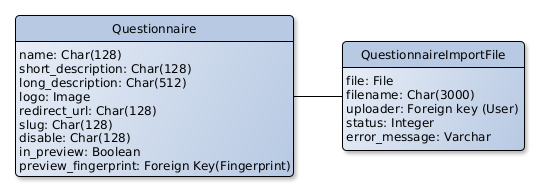
\includegraphics[width=.6\textwidth]{questionnaire-import-models}
    \caption{Questionnaire model and the model where questionnaire imports information is stored.}
    \label{fig:questionnaire-import-models}
\end{figure}

If the questionnaire is valid, the user will be redirected to a page where he can preview the result and can accept or reject it.
It is important to point out that for the preview process a new Fingerprint object is created so \gls{api} calls can be performed.

Strangely on the Questionnaire model, the disable column uses a character type column instead of a boolean one since it expects only the value of ``False'' and ``True''.
If there are some user input errors, it could lead to unexpected behavior or internal server error.

% ---

Associated with how the structure of a questionnaire is stored, there are only four models to do so: Questionnaire, QuestionSet, Question, and Choice.
All are associated with a specific concept of the questionnaire, although other concepts are not represented.
First, there's the category, used to create question groups within a question set.
It is represented as a question record, where the ``category'' field of the question models has the value ``true''.
For more complex question types, that require extra configuration, such as choice tabular (name of the rows and column) and open multiple (name of the columns), such data is stored in a metadata field of the associated question model.
Question types that do not make use of these fields, will have an empty value, leading to some database space being wasted.

\begin{figure}[H]
    \center
    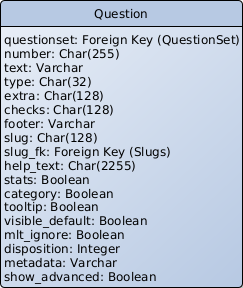
\includegraphics[width=.3\textwidth]{question-model}
    \caption{Question model and its extensive number of fields.}
    \label{fig:question-model}
\end{figure}

When the questionnaire's spreadsheet was explained, some fields were related to some old deprecated features.
The question model contains the same fields that map to the questionnaire's spreadsheet deprecated fields: stats, visible\_default, and disposition.
There is also a slug\_fk field that points to a Slugs model that replicates the question's slug and text, which was used to yet another deprecated feature.

Finally, a question supports for the user to define additional checks which are defined on the ``checks'' field however, this feature is not exposed through the questionnaire's spreadsheet.

\section{Refactoring}
% o que necessita de, ou vai, ser alterado

Until now it was shown how the MONTRA framework was designed around databases, their metadata, and how that metadata can be shared among the platform users.
For regular users the framework provides a good user experience, however, for power users, that make use of \gls{api}s, might make some errors which the framework will not prevent, leading to inaccurate data to be stored and presented.
Also for developers, such flaws and bad design choices make the maintainability process of MONTRA instance a demanding and tedious process.

With this, there is a clear opportunity to perform a refactoring process over the framework to correct such problems and the issues that have been emphasized in this chapter.
The goal of this refactoring process is not to change the framework in a way to transform existing use cases, but to improve its internal structure to make the framework more stable, easier to maintain, and easier for an external tool to communicate with it, mainly to publish database data.

Next, we will propose several changes to be applied to the framework, beginning from the data models, regarding how fingerprint answers data is stored, how questionnaires structure is stored and some other fixes for some defects explained previously.
Such refactoring will imply changes on other components, one of them being the rendering of questionnaires and how input validation is done.
Finally, several clutter problems were mentioned when describing the spreadsheet to define a questionnaire structure, so the spreadsheet will also undergo a refactor.

\subsection{Data Models}
% explicar escolha de apenas reformular apenas a apartir de determinado nivel
% explicar os novos modelos e de que maneiras resolvem problemas que existiam
% trade offs tidos em conta
% diagrama de classes com diferenças

Since the MONTRA framework uses some outdated software and there are active installations, the refactoring process can not be done by simply designing new models and views, implementing them, and replacing old ones is not a viable option.
The approach taken was to first decide what components would go through a refactoring process and within each, until what level we would apply it.

Taking into account figure \ref{fig:old-models}, since both the Community and Developer (Plugins) Django applications target functionalities not so fingerprint-centric and are more related to features of the framework as a whole, we decided not to perform any changes on the models of these applications.
This leaves us with both the Fingerprint and Questionnaire applications.
Regarding the Fingerprint application, the fingerprint model is one of the main models of the framework, affecting several features of the framework, so we intend to perform minimal changes on it.
However, the remaining models associated with the answers of a fingerprint and submissions will have a new model design.
Respecting the Questionnaire application both the Questionnaire and QuestionSet models represent well-defined concepts and do not require any changes.
Yet, the remaining models, mainly the models storing the structure of the questions, their dependencies, choices, etc.\, will also have a new design.

In Figure \ref{fig:new-models} it is presented the new models in light green.
The decided approach to implement these models was to create a new Django application and create all these new models on that application.
This way, the migration process is an iterative process where the framework is always operational since the previous models still exist.
Then with the help of an \gls{ide}, we can search for usages of the old models and migrate each feature at the time.

\begin{figure}[H]
    \center
    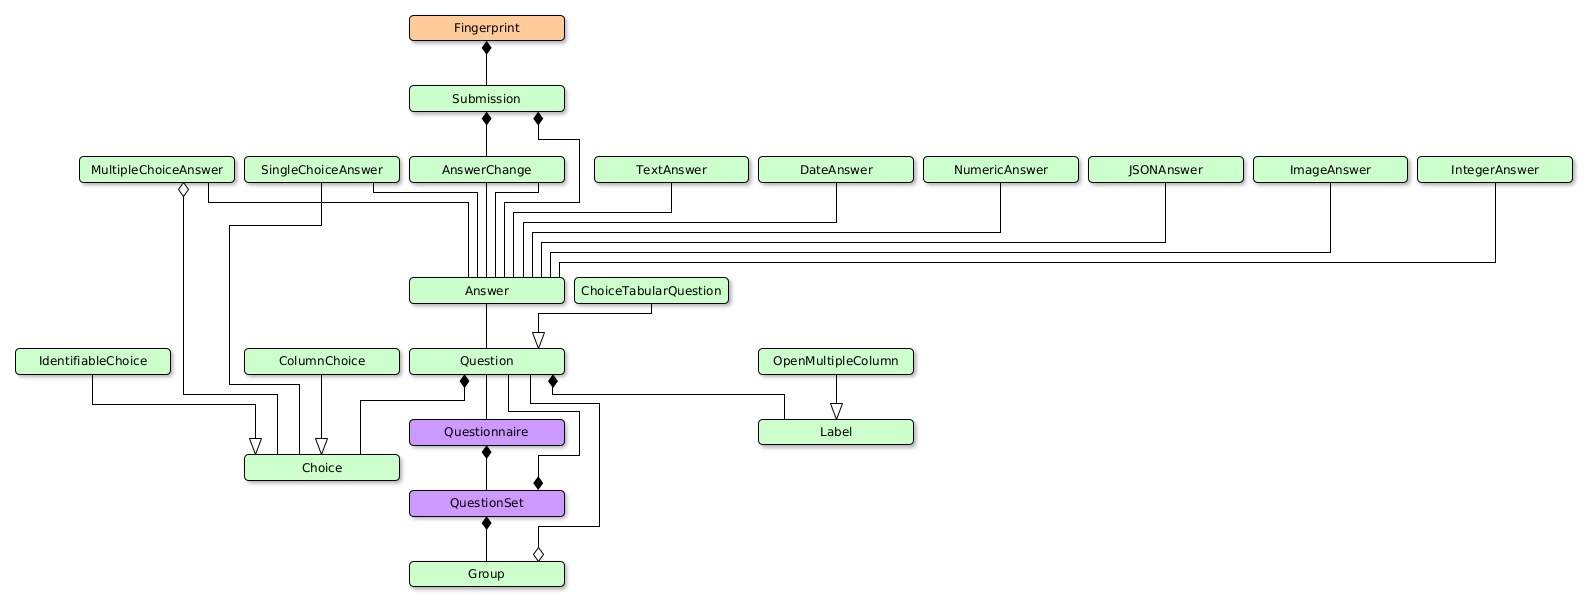
\includegraphics[width=\textwidth]{new-models}
    \caption{Model Diagram of the new models.}
    \label{fig:new-models}
\end{figure}

Let's start with the fingerprint-related changes.
Now there is a new Answer model that does not hold directly the content of answers, instead the content is stored on data-specific models such as IntegerAnswer and DateAnswer.
For choice-based questions, instead of storing the value of the selected choice(s), a single or multiple choice answer contains a foreign key(s) for the selected choices.
To establish the connection between the main Answer model and the data-specific model, the main model contains a \textit{type} field that indicates the data type of the answer.
Then the primary keys of the data-specific answer model are the same as the associated record of the Answer model, which allows fetching the data-specific answers of an Answer.
Is important to note that the number of different answer types is not the same as the number of question types.
Answers of different questions types can be stored in the same answer type models, for example, open text and email questions both can be stored as text in the database.
Previously fingerprint submissions were being represented with the model FingerprintHead, now we created a Submission model which contains the same relationships as before, a set of answers, a set of answer changes, all this associated with a fingerprint.
The AnswerChange model now does not contain the data of the previous and current answers, instead, it contains the foreign keys for the answer model.
In cases where the change was from or to an empty answer, either the previous answer or the next answer field are filled with the NULL value.

Moving now to the models related to the Questionnaire application, there is a new Question model mainly because the previous one had too many fields.
An example of these extra fields is the \textit{metadata}, which is used to store the information of the column of the open-multiple question type and the choices and answering items of a choice tabular question type.
This field was replaced by the addition of new models (Label) which will be explained in more detail in the next Excel subsection.
Another example was the category field, which indicated if a specific question record described a category in the questionnaire which was being used to create subgroups of questions.
With the new models, a new Group model was created which has a set of questions associated.
Previously this relationship did not exist, so MONTRA would create a group based only on the question's order and level.
Additionally, with the addition of this Group model, there is no need to have a level field on the question model, since nested levels are represented through Groups, which can have a parent group.
A group with no parent is represented in the root level of the questionnaire.
The remaining models (Label, Choice, and their descendants) will be explained in more depth in the next Excel subsection since they were created mainly because of how questions are represented in the new spreadsheet format.

Meanwhile, there are previously existing models that have undergone changes to fix some design flaws mentioned before.

\begin{itemize}
    \item QuestionnaireImportFile: To provide feedback to the user this model only contained an \textit{error\_message} field.
        However several times there are some errors with the questionnaire, but the framework can continue.
        In these situations, a warning could be sent to the user just so he is aware that a part of the spreadsheet has some errors and the result could not be his real end goal.
        Then the new model contains two new fields, \textit{errors}, replacing the old \textit{error\_message}, and \textit{warnings} fields, which are stored in \gls{json}, where the keys are the lines where the errors or warnings were found and the values are an array of messages associated with that line;
    \item Questionnaire: associated with the questionnaire model we mentioned that it had a specific fingerprint attached that was used to show a preview of the result of the questionnaire.
        This field is not required since the preview mode of a questionnaire is viewed on read-only, so no answers are associated with these preview fingerprints;
    \item QuestionSetPermissions: From this model, we removed the useless permission of ``Allow Printing'', considering it is impossible to restrict users from printing the page since a screen capture software can be used as a replacement for the browser's print function.
        Also, there was a record associated with each question set of every fingerprint, even if the values of each permission were the default ones.
        The new approach taken is to only create a record if any permission value is different from the default one.
        Otherwise, an object with the default values is returned;
    \item Fingerprint: It has a new ``submission\_token'' used for the new \gls{api} endpoints explained next.
\end{itemize}

\subsection{Views}

When the MONTRA framework was presented it was highlighted that the different variations of the fingerprint view (create, show, edit, search, preview) were all using a different Django template.
Once again, this brings the problem that one change will entail that the same change has to be applied on the remaining fingerprint view variations.
On the refactoring process, these views were adapted so all the different pages use a shared fingerprint template which then renders the necessary components according to the page where are being rendered.

The first step of this process is to put different components into separate templates, which will then allow the creation of different arrangements of such components according to the fingerprint view variation being displayed.
Note that even within these new separate components, some parts of them might be rendered differently according to the fingerprint view variation where they are being inserted into.
In figures \ref{fig:fingerprint-new} and \ref{fig:fingerprint-show-detailed} we can see that some components are present on both views.
The question set title, the questions, the question set menu, the fill progress bar, and the navigation buttons.
However, we can also see some components in figure \ref{fig:fingerprint-show-detailed} which are not present on the on figure \ref{fig:fingerprint-new} such as the fingerprint statistics (hits, unique views and fill percentage), there are no fingerprint-related buttons, which are now questionnaire-wide buttons.
Note that the name of the fingerprint (DemoAveiro), the several tabs (Fingerprint, Documents, etc.) and the subscribe and Manage buttons are specific to the show Page.
The new fingerprint template will only contain components to display within the Fingerprint tab.

In Figure \ref{fig:fingerprint-other-after-diagram} is presented a two-column layout for the create, edit, search and preview variations of the fingerprint view.
Although, some components are not displayed in certain variations, such as the Cancel and Save buttons.
The Cancel button is not displayed on the preview variation, and both Cancel and Save buttons are replaced by a Search button.
Additionally, different buttons appear on the question set buttons component according to the fingerprint view variation.

\begin{figure}[H]
    \center
    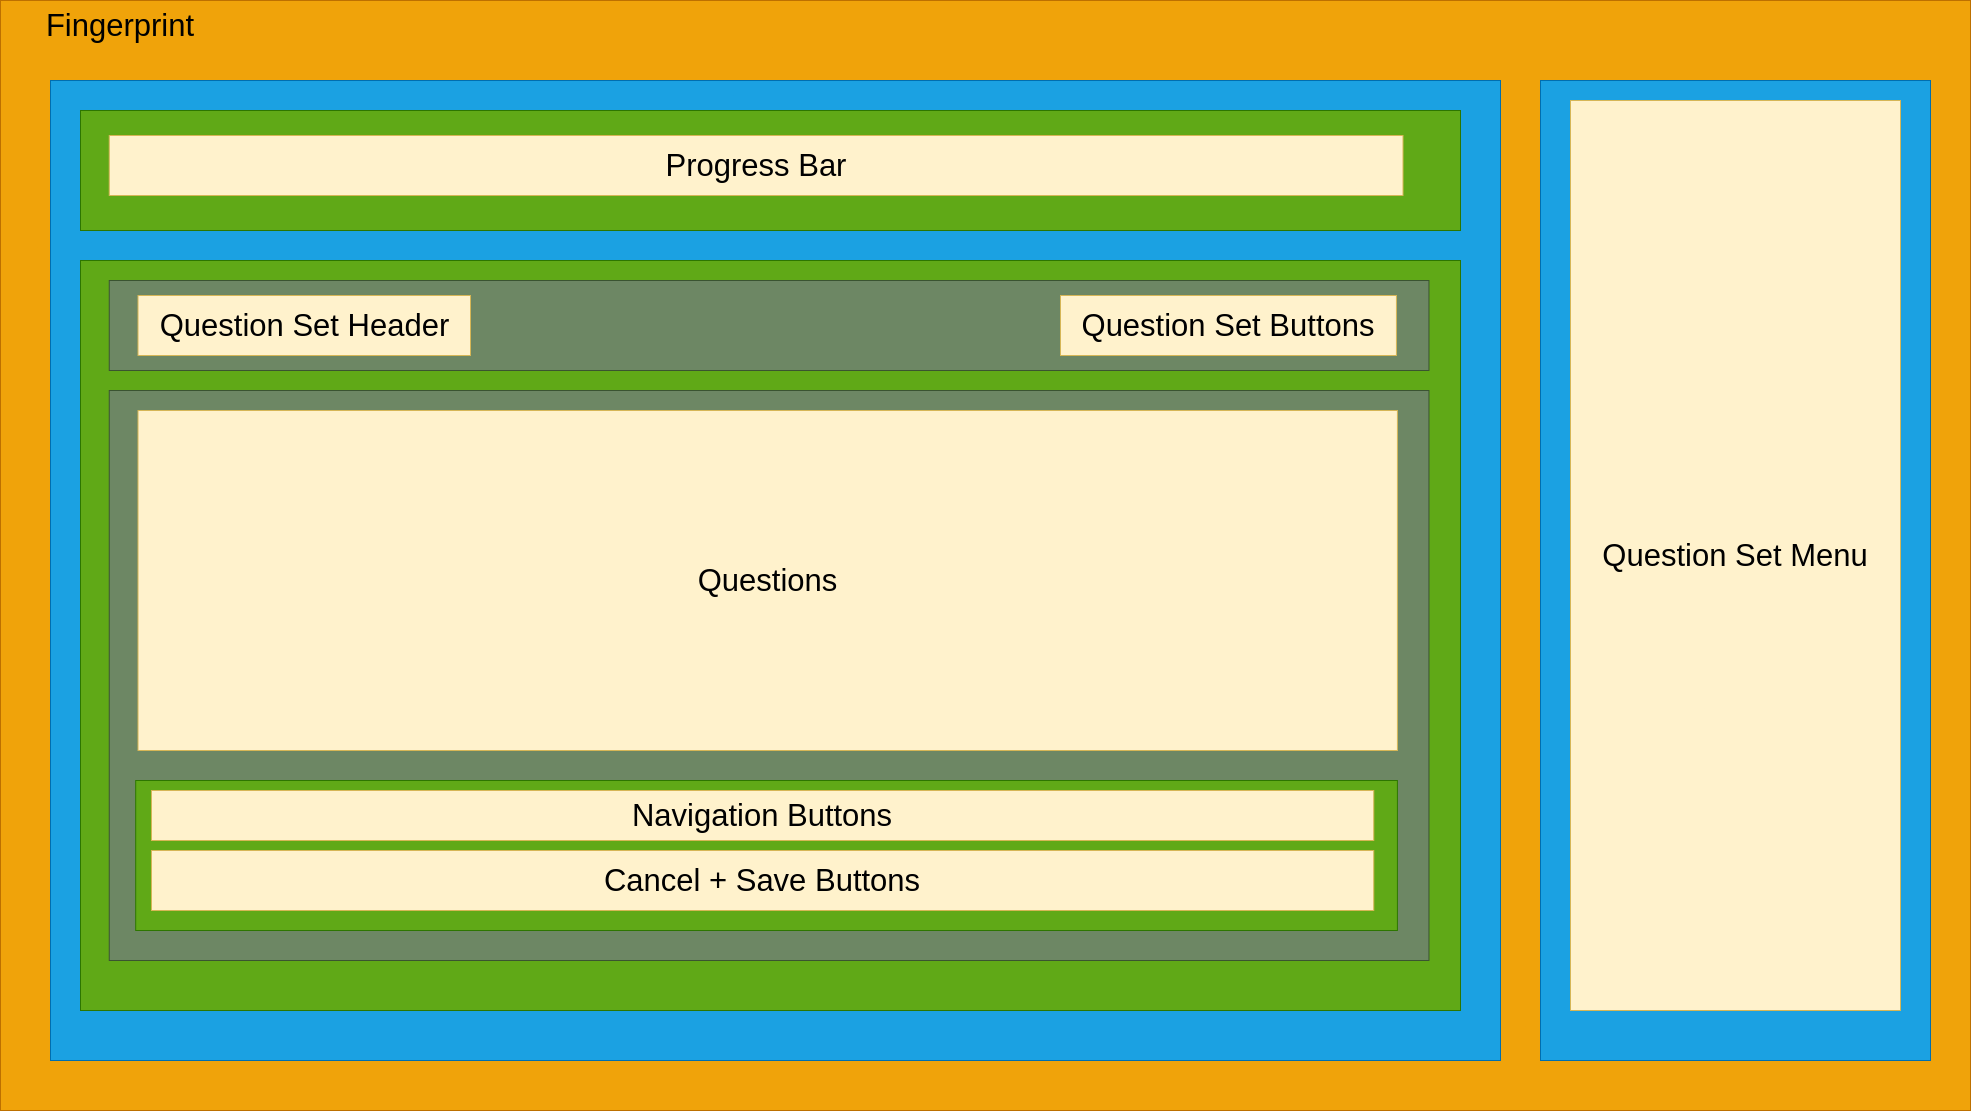
\includegraphics[width=\textwidth]{fingerprint-other-after-diagram}
    \caption{New fingerprint template for the create, edit, search and preview fingerprint views variations.}
    \label{fig:fingerprint-other-after-diagram}
\end{figure}

The show variation, as shown in figure \ref{fig:fingerprint-show-detailed-after-diagram}, uses a single column with two rows layout.
Previously the show variant had no Question set buttons, however, to keep consistency with the other variants, the Collapse and Show buttons were moved to the Question Set Buttons where they were being displayed on the other variants.
By default, the only button visible on the Questionnaire buttons is the Summary, which will hide the current detailed view and show an alternative summary layout, where answers are displayed in several tables, one for each question set.

\begin{figure}[H]
    \center
    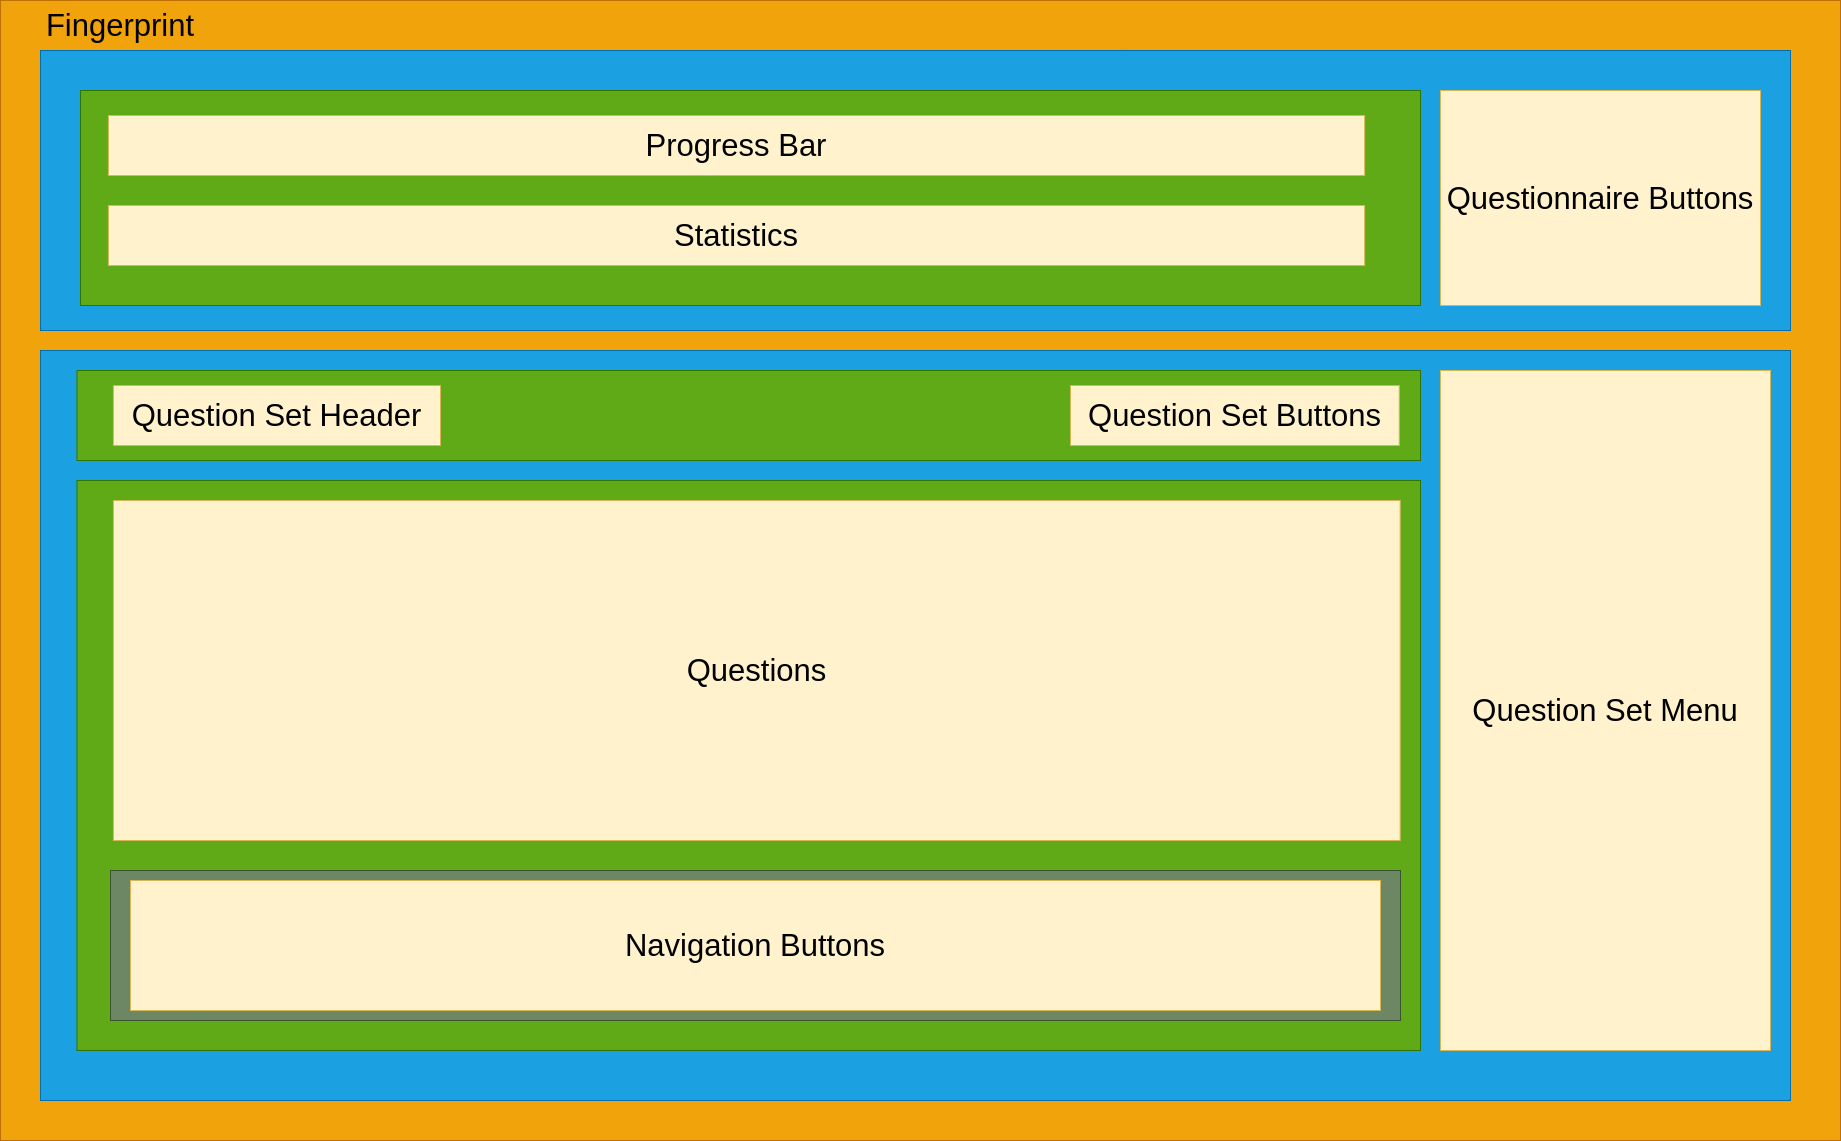
\includegraphics[width=\textwidth]{fingerprint-show-detailed-after-diagram}
    \caption{New fingerprint template layout for the detailed show fingerprint view variation.}
    \label{fig:fingerprint-show-detailed-after-diagram}
\end{figure}

As can be observed in figure \ref{fig:fingerprint-show-summary-after-diagram}, when the user switches to the summary view, by clicking on the Summary Questionnaire button, the detailed view container is hidden, and the summary view container is displayed.

\begin{figure}[H]
    \center
    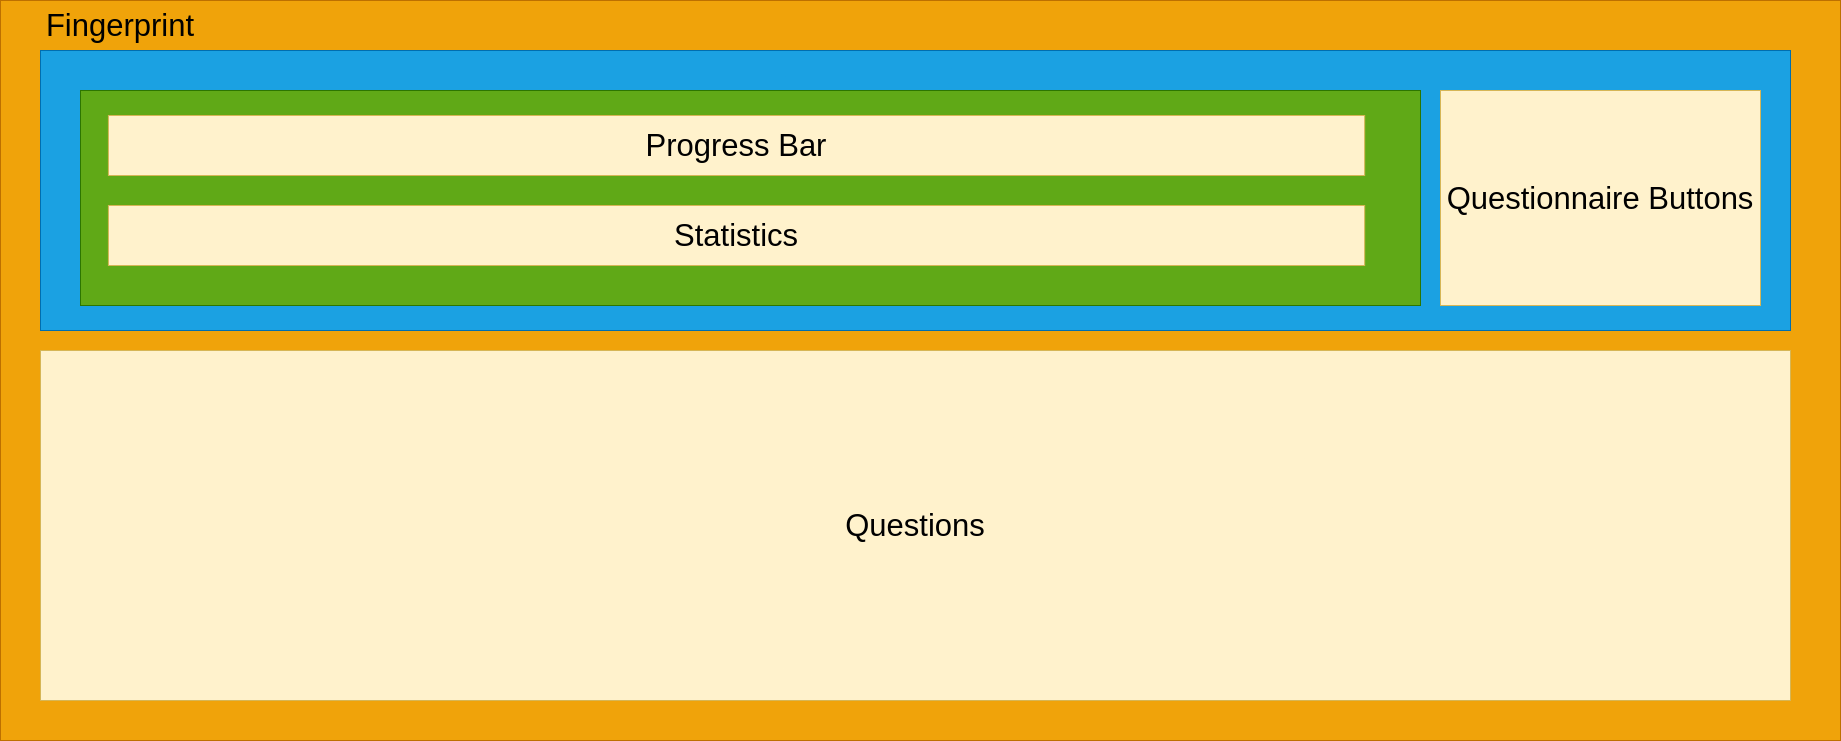
\includegraphics[width=\textwidth]{fingerprint-show-summary-after-diagram}
    \caption{New fingerprint template layout for the summary show fingerprint view variation.}
    \label{fig:fingerprint-show-summary-after-diagram}
\end{figure}

It is important to note again that the overall aesthetics and workflow of the page were not changed.
The only major change was to divide the fingerprint view into several, reusable components.

When we went over how question sets were rendered, we saw that each question set had its container and they are only rendered when is accessed for the first time.
When it needs to be rendered, \gls{api} endpoints are used to fetch the \gls{html} of a specific question set.
On this \gls{html} returned, each question had attached their client-side validation code.
The goal is to remove all existing code of client-side validation, making use of only simple built-in \gls{html} validations on the client-side and use Django's forms framework to have all remaining validations on the server-side.

Before going into more details let's go over Django's built-in form system and some of its components.
A form in \gls{html} is represented through the form tag and fields are represented through input tags.
Each input tag has a type attribute that defines how the data will be inserted by the users, for example, to insert a date the user will be presented with a calendar where it can click on the desired date.
These different ways to insert data are called widgets.
To work with forms, Django only makes use of two \gls{http} request methods: GET and POST.
GET is used by browsers to fetch the page/\gls{html} of an URL and it can also be used to fetch information.
POST on the other side is used to send information to a server.
On the backend side, Django has three main classes that handle the data around forms.
The main one is the \textit{Form} class that defines how it works and how it will be presented to the user.
Then there is the \textit{Field} class that describes a field of a form, which is in charge of performing field-specific validations.
Django already has some implementations of this class for the most common field types such as number, text, choice, etc.
Finally, the \textit{Widget} class is in charge of processing and transforming the raw data received and also preparing and restructure data to be presented to the user, and again Django already has some implementations of this class.
Each \textit{Field} class has a widget class associated.
The common development flow is to create a child class of Django's \textit{Form} class and then define its fields with \textit{Field} classes.

However, in the case of MONTRA, the number and type of the fields are dynamic, since both can be customizable by a community manager when he is building a questionnaire.
A Submission form was created, child of Django's \textit{Form} class, where its constructor was overridden so the fields of the requested Question Set of a Questionnaire are defined in the form class.
Additionally, several question types lead to the need of having to create and associate new \textit{Field} and \textit{Widget} child classes since they were too complex to be represented or validated with the ones that Django already has implemented.
To build the widgets of such question types, existing implementations were ported to an associated Django template to then be used in its new widget class.

By removing all validations from the front end, client-side code is now only used to make \gls{api} calls to the backend to validate the data inserted by the user, and to add functionality to the page itself, such as hide and/or show elements on the page after a button is clicked.
All client-side code related to the fingerprint was either migrated or newly implemented using, as much as possible, plain javascript, avoiding any external library.
It avoids adding yet another dependency to the project, and if in the future, upgrades are done to libraries such as JQuery\footnote{https://jquery.com/}, the code implemented here is not affected and does not require any refactoring.

\subsection{Programming interface}
% UI changes
% consequencia da alteração do front end devido à alateração do backend
% passar toda a verificação para o backend, passando a usar a validação built in do Django
% tentar reutilizar os modulos existentes

As all the validations were moved to the backend, it was necessary to create several \gls{api} endpoints that perform them.
Such validations take advantage of Django's form system, so in the implementation of each endpoint, it is only necessary to build a SubmissionForm then add the data provided by the user and then call its validation method, which will validate all the fields that were defined in the form.

Besides the user input validation, there needs to be new endpoints that render the \gls{html} of a question set of a questionnaire using the new questions models and Django's forms system.
As different fingerprint view variations might present the questions and answers differently, there are different endpoints for each fingerprint variant:

\begin{lstlisting}[basicstyle=\tiny]
GET  [base url]/questions/[questionnaire id]/[section index]/preview/

GET  [base url]/questions/[community slug]/[questionnaire id]/[section index]/search/

GET  [base url]/questions/[community slug]/[questionnaire id]/[section index]/create/
GET  [base url]/questions/[questionnaire id]/[section index]/create/

GET  [base url]/questions/[fingerprint hash]/[section index]edit/

GET  [base url]/questions/[fingerprint hash]/[section index]/show/
\end{lstlisting}

There are two different endpoints for the create variant, because certain installations are a single community, for that, the community is implicit, but for multi-community installations, the community slug is required, since the same questionnaire can be used on different communities.

For the edit and create variants, there need to be additional endpoints that are in charge of performing all the validations associated with each field and saving the progress when the user changes from one question set to another if no error is found.
Bellow are such:

\begin{lstlisting}[basicstyle=\scriptsize]
Submissions Management:
POST [base url]/api/submission/save/[community slug]/[questionnaire id]/[section index]/
POST [base url]/api/submission/save/[questionnaire id]/[section index]/
PUT [base url]/api/submission/save/[fingerprint hash]/[section index]/
\end{lstlisting}

Related to the Submissions Management endpoints, which are used to save answers data, the first two endpoints follow the same idea as the ones presented before, which on single community installations there is no need to provide the community slug.
However, there is a third alternative.
The first two should be used when there is not yet a fingerprint created, and which will return both the fingerprint hash of the created fingerprint and the current submission token.
The fingerprint hash is the identifier of a fingerprint, the submission token is used to identify if different calls to the save endpoints are related to the same changes.
With that, several changes can be grouped in the same Submission, instead of the previous implementation that would create a FingerprintHead record for each save of a question set.

This also enforces that if the user performs several changes to the same question set with the same submission token, only the last changes will be kept, replacing (figure \ref{fig:submissions-new-answer2}), or even deleting (figure \ref{fig:submissions-remove-answer}), old answer values sent in the same submission.

\begin{figure}[H]
    \center
    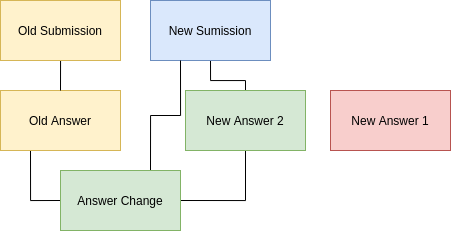
\includegraphics[width=.5\textwidth]{submissions-new-answer2}
    \caption{When an answer change is submitted and there were already changes made to that question, then the previous one is deleted (New Answer 1) and a new one (New Answer 2) is associated with both the current Submission and the related Answer Change.}
    \label{fig:submissions-new-answer2}
\end{figure}

\begin{figure}[H]
    \center
    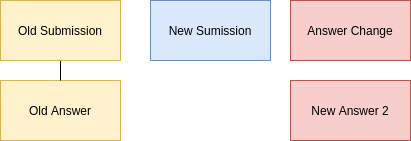
\includegraphics[width=.45\textwidth]{submissions-remove-answer}
    \caption{If the user either provides an empty value or no value to an answer that previously had a value on the current submission, associated Answer and Answer Change records are deleted.}
    \label{fig:submissions-remove-answer}
\end{figure}

If no submission token or one that does not match the current one is provided, then it is assumed that the changes submitted are related to a new submission, thus the most recent submission is closed and the new provided answers are added to a new submission.

\begin{figure}[H]
    \center
    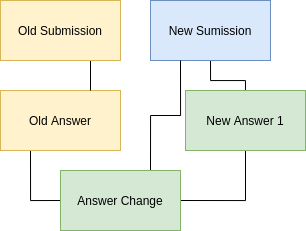
\includegraphics[width=.3\textwidth]{submissions-new-answer}
    \caption{Whenever new changes to the answer of a question in a specific submission are submitted, a new Answer model is created, and also an Answer Change record is created connecting with the previous answer.
In the case the provided submission token does not match the current one stored in the fingerprint model, then a Submission record will also be created, and changes will be associated with this new Submission.}
    \label{fig:submissions-new-answer}
\end{figure}

Previously it was possible to update an answer of a single question through endpoint \textit{/api/fingerprints/[fingerprint hash]/answers/[question slug]/}, mentioned in the \gls{api} portion of section \ref{sec:fingerprints}, which was a more user-oriented alternative to the ones that were used on the old fingerprints views.
On the new endpoints to validate and save the answers of a question set, if a single answer is sent, Django's form system will consider the rest of the answers to the other questions of the question set as empty.
With this, the user is forced to always send the previous answers to all other questions plus the updated answer of the specific question.
To avoid this, the \textit{/api/fingerprints/[fingerprint hash]/answers/[question slug]/} endpoints were kept, refactoring them to use the new models and Django's form system, but in these, the form used to perform the validation only contains one question instead of all questions of a question set.

With all this changes to the endpoints, choice-based answers are stored as a foreign key to the choice(s) selected.
This implies that the answer's data sent on the Submissions Management endpoints for such question types must be these foreign keys, avoiding misspellings and non-existing choices.
However, one does not know the keys for each choice and also the available choice if the web view is not used.
For that, the Questionnaire Information endpoints are used to get information of choice-based questions, so that the correct data is sent along with the Submissions Management endpoints.

\begin{lstlisting}[basicstyle=\scriptsize]
Questionnaire Information:
GET  [base url]/api/questionnaire/info/[community slug]/[questionnaire id]/[section index]/
GET  [base url]/api/questionnaire/info/[questionnaire id]/[section index]/
\end{lstlisting}

\subsection*{Draft Status API}

There were also some modifications to the endpoints to change the publish status of a fingerprint.
Instead of having two different endpoints for different community settings (to auto-accept or not fingerprint publish requests), but for the same purpose, now only one exists.

\begin{verbatim}
POST [base url]/api/draft/[fingerprint hash]
\end{verbatim}

This endpoint expects the same data in the same format, though takes different actions according to the community of the fingerprint at issue.
Also, on the previous versions of publishing endpoints, there was a possibility to publish fingerprints that were not complete, not having answers to required answers.
Now, a validation is implemented when the user wants to publish its fingerprint, not completing the change on the publish status if the fingerprint is not complete.
This avoids notifications being sent to the community manager telling that a user wants to publish a fingerprint, although such fingerprints might be incomplete.

\subsection{Excel}
% mais concreto, e tem mais em conta o contexto em volta das questoes
% entanto é mais estenso
% tipos de perguntas novos e deprecated

The previously presented version of the spreadsheet used to define a questionnaire, had some problems in terms of clutter due to the overuse of the ``Value list'' column to define the extra configuration of specific questions types.
The column was used to define all choices and their extra information of choice-based questions, to define columns and their settings of open multiple question and columns, rows, and type of choice tabular questions.

To fix those clutter problems, improvements were done to the spreadsheet by deleting some useless columns that were related to deprecated features and adding new types of rows that define the extra configurations for those questions types that require it.

Starting by the columns of the actual spreadsheet, now are the following:

\begin{itemize}
    \item Type;
    \item Text/Question;
    \item Level;
    \item Data Type;
    \item Help Text/Description;
    \item Slug;
    \item Dependencies;
    \item Constraints;
    \item Tooltip;
    \item Include in Advanced Search.
\end{itemize}

Most of the columns are already known from the previous version, ``Constraints'' being the only one that was added to this new version.
The columns that were removed are Stats, Comments Stats, Disposition (all associated with deprecated features), Level/Number (the number is now automatically retrieved according to the order of how the rows are defined), and Value List (brought the clutter problem to the table).

\subsection*{Type}

On this column, the only possible values available were QuestionSet, Question, and Category.
The new version has now eleven possible types of rows for the spreadsheet:

\begin{table}[H]
\centering
    \begin{tabular}{| p{.2\linewidth} | p{.8\linewidth} |}
\hline
\textbf{Type}                 & \textbf{Description}                                                                       \\ \hline
\multirow{2}{*}{IntroSection} &
  \multirow{7}{=}{These represent the same concept as QuestionSet. \\ In the previous version, it was possible to add hidden question sets to both the beginning of the end of the questionnaire. This was achieved by setting the Level/Number column to either 0 or 99 respectively. Since the Number portion of that column was removed, such Question Sets must be represented with the IntroSection and CloseSection rows.} \\
                              &                                                                                            \\ \cline{1-1}
\multirow{3}{*}{Section}      &                                                                                            \\
                              &                                                                                            \\
                              &                                                                                            \\ \cline{1-1}
\multirow{2}{*}{CloseSection} &                                                                                            \\
                              &                                                                                            \\ \hline
Group                         & This is a replacement to the category row type plus the comment question type.             \\ \hline
Question                      & The old and unchanged Question row type                                                    \\ \hline
Choice                        & This row indicates a choice of the previously defined Question                             \\ \hline
ChoiceInfo &
  Allows adding an extra question that can be answered if a specific choice is selected. Such a question will be rendered right below the choice.

        Note that this is different from the dependencies column. \\ \hline
TabularChoice                 & \multirow{2}{*}{Row types to define the configuration of choice tabular question types}    \\ \cline{1-1}
TabularRow                    &                                                                                            \\ \hline
Column                        & \multirow{2}{*}{Row types to define the configuration of the open multiple question types} \\ \cline{1-1}
ColumnChoice                  &                                                                                            \\ \hline
\end{tabular}
\caption{Available values to use on the ``Type'' Column of the new version of the spreadsheet to define a questionnaire.}
\label{tab:excel-row-types}
\end{table}

Using the new row types described in table \ref{tab:excel-row-types}, the spreadsheet itself will be longer, however, it will be easier to read.
In figures \ref{fig:choice-tabular-neu}, \ref{fig:open-multiple-neu} and \ref{fig:choice-neu}, it is presented three before and after of how questions that require extra configuration were and are now defined with the new spreadsheet version.

\begin{figure}[H]
    \center
    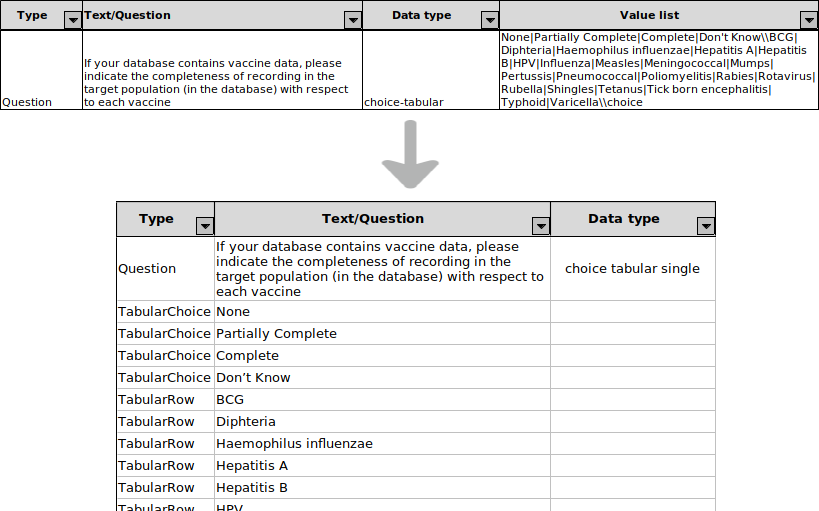
\includegraphics[width=.75\textwidth]{choice-tabular-neu}
    \caption{Differences between how a choice tabular question was versus how is now defined on the questionnaire spreadsheet.}
    \label{fig:choice-tabular-neu}
\end{figure}

\begin{figure}[H]
    \center
    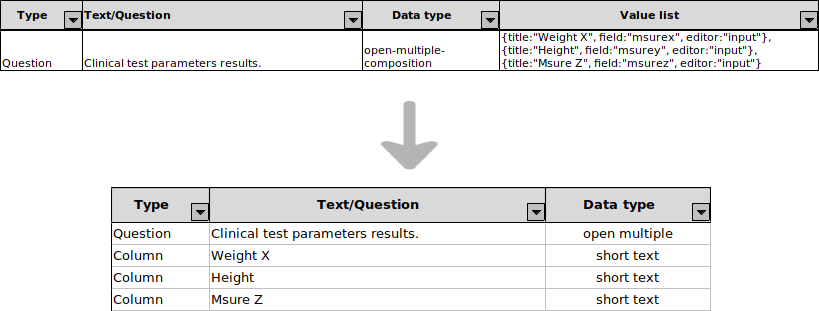
\includegraphics[width=.75\textwidth]{open-multiple-neu}
    \caption{Differences between how a open multiple question was versus how is now defined on the questionnaire spreadsheet.}
    \label{fig:open-multiple-neu}
\end{figure}

\begin{figure}[H]
    \center
    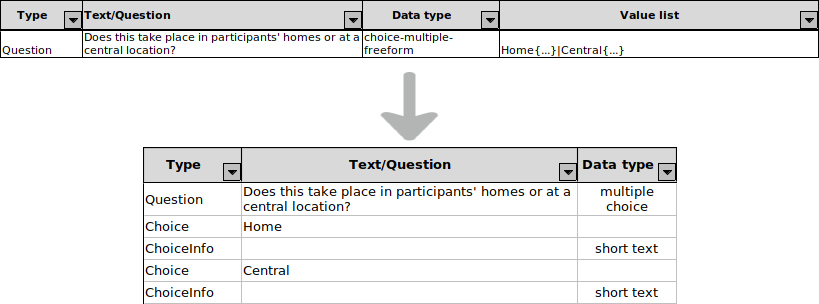
\includegraphics[width=.75\textwidth]{choice-neu}
    \caption{Differences between how a open multiple question was versus how is now defined on the questionnaire spreadsheet.
    Note that now it is possible to specify the data type of the extra information that is attached to the extra information of a choice.}
    \label{fig:choice-neu}
\end{figure}

It was considered to also remove the Level part of the Level/Number column, adding an EndGroup row type.
Then whenever the user wanted to create a subgroup of questions after a question would create a Group with empty text and the framework would move the question of that group to a deeper level with no group label.
This however would make the spreadsheet even longer for certain questionnaires that make use of categories to group questions that have some dependency on another question.
Figure \ref{fig:excel-end-group} shows how the change would affect the spreadsheet.

\begin{figure}[h]
    \center
    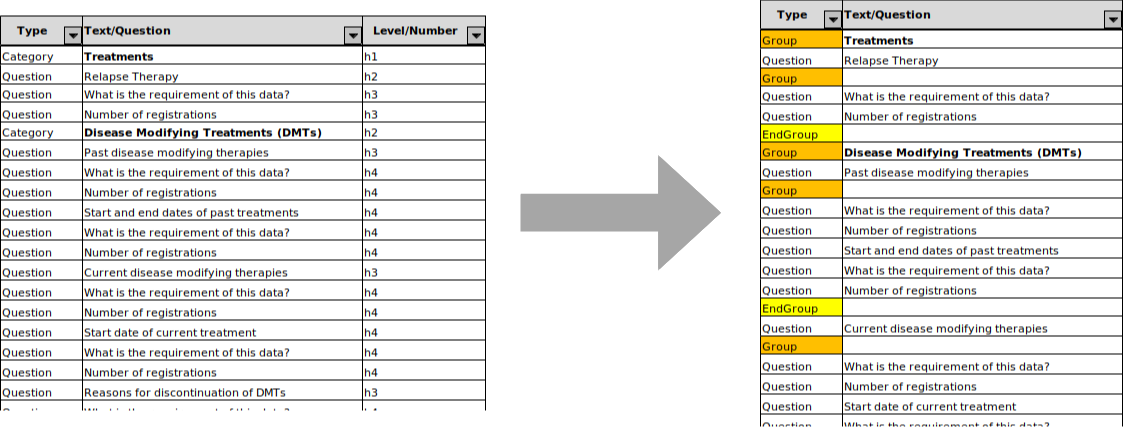
\includegraphics[width=\textwidth]{excel-end-group}
    \caption{A possible solution to avoid relying on the Level column to create subgroups of questions. On the new solution proposed it is much difficult to know at which level the specific question is located, without looking at the rows above.}
    \label{fig:excel-end-group}
\end{figure}

Even with colors, the user editing has to look several rows above to know at each level it is so he can match the ``EndGroud'' rows with the respective ``Group'' rows.
This is the same problem as matching if open and closing brackets on C-like programming languages.
Such a problem is alleviated on them since indentation is allowed, which can not be achieved on a spreadsheet.
For those reasons, the Level column was kept, however, when a questionnaire is imported, whenever there are nested levels the framework will create groups with empty text.

\subsection*{Data Type}

As it was possible to see in figures \ref{fig:choice-tabular-neu}, \ref{fig:open-multiple-neu} and \ref{fig:choice-neu}, the Data Type column is used to detail the type of data that will be stored and how it will be requested to the user in terms of HTML widgets.

Table \ref{tab:original-question-types} contains all the previously allowed question types, a total of twenty-five different types.
On the new version, this list was reduced, where some questions can now be achieved using simple question types in conjunction with the new row types that extend their base functionality.

Next is the list of question types available after the refactoring:

\begin{itemize}
    \item short text: Old open. It replaces the open-validated field by making use of the new Constraints column;
    \item long text: Old open-textfield;
    \item single choice: Used to achieved any old single-choice question type. The extra information input can now be achieved with the ChoiceInfo row type;
    \item multiple choice: Used to achieved any old multiple-choice question type. The extra information input can now be achieved with the ChoiceInfo row type;
    \item integer: Old integer;
    \item date: Old datepicker;
    \item email: Old email;
    \item url: Old url;
    \item numeric: Old numeric;
    \item publication: Old publication;
    \item image: Old open-upload-image;
    \item choice tabular: Old choice-tabular;
    \item open multiple: Can achieve both the old open-multiple and open-multiple composition.
\end{itemize}

Open-location and timeperiod were removed since they were not being used on any of the active installations of the MONTRA framework.
The same happened with sameas and custom as additionally, they were shortcut type questions.

\subsection*{Slug and Dependencies}

Previously the dependencies between questions were detailed by providing the id of the target question and the order of the choice that was needed to be selected, but since now the choices are described by row, the user can also detail an id for them, which such id can then be used on the Dependencies column of the questions that depend on such choice.

\subsection*{Constraints}

The old Question model allowed to add custom checks, however, this feature was not possible to make use of through the spreadsheet, it was only possible to define them after the questionnaire was imported.
This ``Constraints'' column intends to enable configuring such additional checks.
Checks were previously stored in a custom format, where each check was separated by a space, defined as $name="value"$.
To avoid having to parse a string every time we want to load the constraints, they are now stored in a \gls{json} field.
Regarding the spreadsheet, the format chosen was a modified version of the original checks format, supporting several types instead of interpreting every value as a string, allowing flexibility on the whitespace between each and within a check.
Next is presented some examples:

\begin{verbatim}
name: "value"  -> string
name: true     -> boolean
name: 1        -> integer
name: 1.5      -> numeric
name: value2   -> also a string
\end{verbatim}

\gls{json} was also considered, however it was too much verbose to put on a spreadsheet cell, emerging the clutter problem.

Currently, the supported constraints are the following:

\begin{table}[H]
\centering
\begin{tabular}{|l|l|}
\hline
\textbf{Question Type(s)}                                                       & \textbf{Constraint} \\ \hline
any                   & required    \\ \hline
\multirow{3}{*}{\begin{tabular}[c]{@{}l@{}}short text\\ long text\end{tabular}} & min\_length         \\ \cline{2-2}
                      & max\_length \\ \cline{2-2}
                      & regex       \\ \hline
\multirow{2}{*}{\begin{tabular}[c]{@{}l@{}}integer\\ numeric\end{tabular}}      & min\_value          \\ \cline{2-2}
                      & max\_value  \\ \hline
\multirow{3}{*}{date} & min\_date   \\ \cline{2-2}
                      & max\_date   \\ \cline{2-2}
                      & format      \\ \hline
\end{tabular}
\caption{Newly available constraints to apply to a question.}
\end{table}


\section{Summary}
In this chapter, a metadata storing and visualization tool, the MONTRA framework, was detailed and analyzed, highlighting some of its poor design choices, which impact its usability and maintainability.
A refactoring process was performed to fix such problems, preventing and giving feedback on user error when submitting data and improving the overall maintainability of components related to the metadata displaying.

The next chapter will go over the remaining part of the process regarding metadata.
Extracting it from a database and then send it to update tools that store and display it, such as an installation of the MONTRA framework.
